\textit{Manuscript in preparation.}

\section{Drug discovery and development: challenges and opportunities.}
Drug development is the process of synthesizing a new chemical entity to treat a specific condition or to control its symptoms. Since \textit{Galen} to modern medicine, the advances in the understanding of human biology and the development of new technologies fuelled great drug discoveries and drove paradigms shifts in the conception of novel therapies \cite{drews2000drug,knowles2003target}. The process starts with identifying a target, such as membrane receptor proteins, then a set of candidate small molecules are either designed or selected from compound libraries \cite{cook2014lessons,willmann2008molecular}. The best performing molecule in animal models, the candidate, is further optimized for improved pharmacokinetic properties. The candidate is then translated for first-in-human trials where the compound is tested on a small set of healthy volunteers to investigate potential human activity. In the second phase of clinical trials, patients are included in the trials to further assess the safety and efficacy of the drug. In Phase III, the cohorts are enlarged to include a greater number of volunteers in randomized controlled multicenter trials to assess the added value of the drug in clinical practice. After marketing, the drug is monitored and the side effects are reported by clinical practitioners to national health agencies and to the manufacturer \cite{wise2009new} (Figure \ref{fig:ddprocess}).\\
In 1997, the average cost of putting a molecule on the market was 500 million dollars \cite{rawlins2004cutting,dimasi2003price}. In 2014, 2.6 billion dollars are required to successfully market a drug \cite{mullard2014new,dimasi2016innovation}. Despite the increasing costs, the process is subject to high attrition rates \cite{cook2014lessons}. In fact, one in 57 programs will succeed in providing a novel therapeutic alternative. In 2016, the Food and drug administration (FDA) approved only 18 new drugs ( New molecular entities (NMEs) and Biologics license application (BLAs)) in the worst rate since 2007 \cite{mullard20172016}. The causes of failure were attributed at 56\% to the efficacy of the drug and 28\% to its safety. Moreover, a recent study showed that two thirds of antineoplastic drugs approved by the European medicine agency (EMA) between 2009-2013 failed to show an improvement over existing therapies \cite{davis2017availability}.\\
The high attrition rates are attributed to poor understanding of disease and drug mechanism. The candidate molecule is often translated to clinical phases solely based on efficacy in rodent models, or on high structural specificity towards the target, often overlooking the system as a whole. A classical example surrounds high density lipoproteins (HDL) increasing drugs (Torcetrapib, Dalcetrapib) that were thought to provide a protective effect in cardiovascular disease based on empirical observations linking the increase of HDL to lower events of heart attacks. The molecules failed to provide a protective effect because the decrease of myocardial infarction was later linked to a lowering of low density lipoprotein (LDL) \cite{voight2012plasma}, for which statins have been successfully developed. Furthermore, a recent study showed that drug programs that have a high validation in biology such as human genetics and human biology supporting the target e.g., genome-wide association studies (GWAS), had a success rate in phase II of 62.5\% as opposed to 5.9\% to targets with low validation\cite{keseru2009influence} \cite{hubbard2006structure}. The overall clinical success rate of genetically validated small molecules was  63\% in comparison to 13\% of success rate in traditional small molecules in Phase II \cite{ringel2013does}.\\
\begin{figure}[!ht]
\centering
	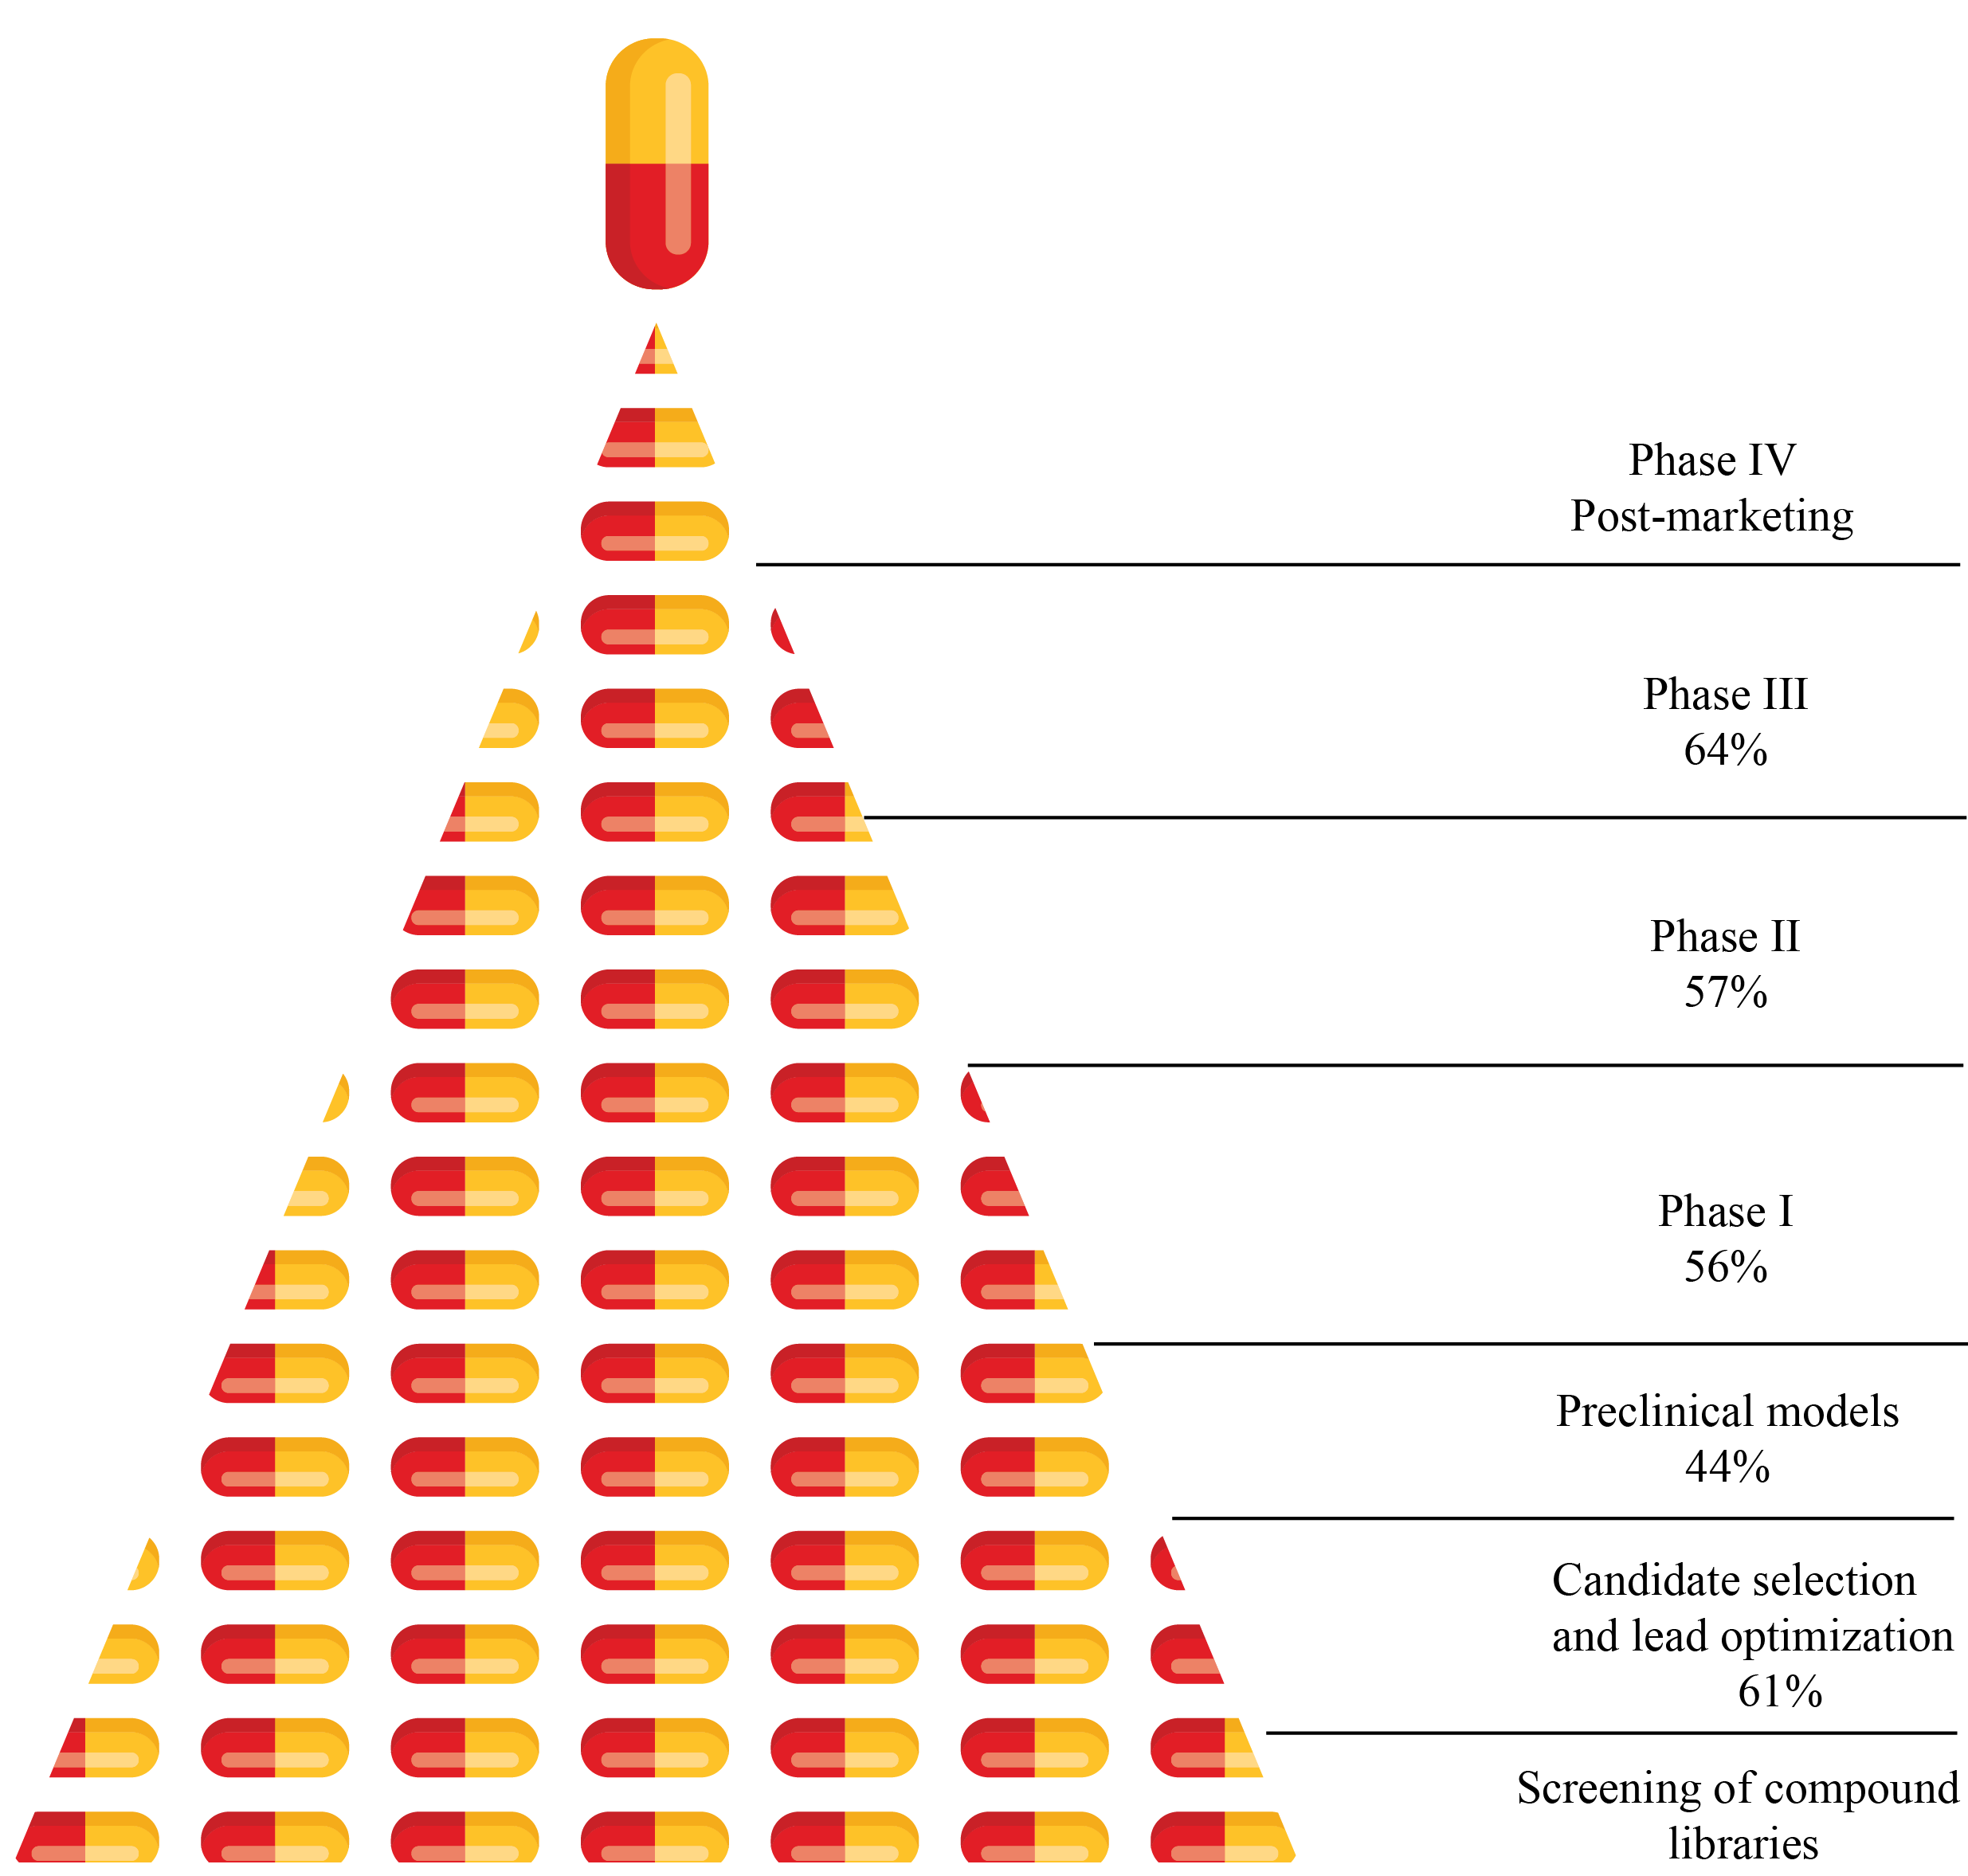
\includegraphics[width=\textwidth,height=\textheight,keepaspectratio]{Intro/ddprocess.png}%Figure from images\Figure1.png
	\caption[The 2.6 billion dollar pill.]{The 2.6 billion dollar pill. The drug development process starts with the screening of compound libraries, of which a set of leads is optimized in PK properties and safety. The candidate is further optimized in preclinical models and translated into clinical phases where the drug is tested on healthy volunteers and patients. After marketing, the drug can be withdrawn if monitoring reveals an imbalanced risk-benefit. Percentages represent the attrition rate in each phase \cite{cook2014lessons}. In total, 1 in 57 drug programs succeeds.}
	\label{fig:ddprocess}
\end{figure}
In the midst of high attrition, high cost, drug development model, biology has turned to a data-intensive field, mainly after the first sequencing of the human genome \cite{lander2001initial}. The leverage of more than 60 years of biochemical literature, combined with whole-genome, high-throughput sequencing enabled to reconstruct human biological systems \textit{in silico} \cite{duarte2007global,thiele2013community}. Metabolism being the support of biomarkers and the endpoint of the central dogma in biology, integrates the preceding genomic, transcriptomic and proteomic information \cite{mardinoglu2014genome,mardinoglu2013integration}. Modelling metabolism through Constraint-based Reconstruction and Analysis (COBRA) \cite{o2015using} allows to identify drug targets in a system-wide manner and to provide testable hypothesis thereby increasing our understanding of disease and drug action. Coupled with targeted experiments, COBRA modelling could provide a bird's-eye view on the system and drive rational drug design where in each of the steps of the drug development process, the model is further refined to answer a specific question at a given point in time.

\section{Constraint-based modelling of large scale human biological networks}
COBRA methods enable the reconstruction of human biological systems through surveying the metabolic reactions in the literature, leveraging biological data in public repositories, or performing genome-wide experiments. The set of reactions obtained are written in a mathematical format as a stoichiometric matrix $S_{(m,n)}$, where the columns are represented by $n$ reactions and the rows are the $m$ metabolites intervening in the biochemical reactions. If the obtained set of reactions is:   
\[ 
\left \{
  \begin{tabular}{ccc}
  Reaction1 & A+B $\rightarrow$ C  \\
  Reaction2 & D+E $\rightarrow$ B  \\
  Reaction3 & 2 C+D $\leftrightarrow$ E \\
  Reaction4 & B+E $\rightarrow$ C \\
  Reaction5 & A $\rightarrow$ E \\
  Reaction6 & C $\rightarrow$ A + E\\
  \end{tabular}
\right. 
\]
the corresponding stoichiometric matrix $S$ is:

\renewcommand{\kbldelim}{(}% Left delimiter
\renewcommand{\kbrdelim}{)}% Right delimiter
\[
  \text{S} = \kbordermatrix{
    & R_1 & R_2 & R_3 & R_4 & R_5 & R_6\\
    A & -1 &  0 &  0 &  0 & -1    &  1  \\
    B & -1 &  1 &  0 & -1 &  0    &  0  \\
    C &  1 &  0 & -2 &  1 &  0    & -1  \\
    D &  0 & -1 & -1 &  0 &  0    &  0  \\
    E &  0 & -1 &  1 & -1 &  1    &  1  \\
  }
\]
In the next phase, the system can be used to investigate the optimal conditions to perform a specific metabolic function, such as carbohydrate metabolism in the liver, the transport of metabolites by the intestinal epithelial cells, or a linear combination of metabolic reactions, such as the basal maintenance metabolism in the muscle. The problem becomes then a linear program (LP), in which the sought metabolic capabilities are formulated as an objective function, under a set of constraints on metabolic reactions to form the following problem:
\begin{alignat}{2}
  & \text{max or min: } &  & c^{T}_{1}v_{1}  \label{intro:eq0}\\
  & \text{subject to: } &  &  \nonumber
                \begin{aligned}[t] \\
                & Sv_{1}=b \\
                & v_{min} \leq v_{1}  \leq  v_{max}
                \end{aligned}
                \nonumber
\end{alignat}
where $c^{T}v$ is the objective function, $c$ is the vector of coefficients of the metabolic reactions in the objective function, $v$ is the vector of metabolic fluxes going through the reactions and the solution to problem \ref{intro:eq0}, $b$ is the change-of-concentration of metabolites in the considered time step, which when set to 0, the system is considered in steady-state and the solution becomes a subset of the null space of $S$ and the problem is referred to as Flux Balance Analysis (FBA) \cite{orth2010flux}. Additionally, a set of bounds are subjected on the metabolic rates of the reactions such that the allowed interval of a given reaction would be between $v_{min}$ and $v_{max}$. For example all reactions but reaction 3 are irreversible, which translates to a $v_{min} \geq 0$, while reversible reaction 3 would have $v_{min} < 0$ and $v_{max} > 0$. 
Solving problem \ref{intro:eq0} would return the optimal theoretical objective $Z_{1}$ for the system under the given constraints e.g., the maximal growth of the cancer cells in a chemically defined medium, and the solution $v$ of metabolic reactions rates achieving the objective. The flux vector $v$ would inform about the pathways involved in disease progression or drug action. 
Practically, problem \ref{intro:eq0} is often under-determined $(m<n)$, the set of solutions achieving the optimal objective is then the Alternate Optimal Solution (AOS) space. Delimiting the AOS space becomes of paramount importance in human biological models as the solutions would be reported as intervals of  metabolic rates rather than single values, thereby increasing the robustness of results. Flux Variability Analysis (FVA) \cite{mahadevan2003effects} allows the characterization of the AOS through performing two linear programs for each i\textsuperscript{th} reaction with a total of $2n$ linear programs as the following:
\begin{alignat*}{2} 
  & \text{max and min: } & & c^{T}_{i}v_{i} \\
   & \text{subject to: }&  & 
   				\begin{aligned}[t] \\
   				& Sv_{i}=b \\
   				& c^{T}_{1}v_{i}=Z_{1} \\
                & v_{min} \leq v_{i} \leq v_{max}
                \end{aligned}
\end{alignat*}
,where $c^{T}_{i}$ has one in the i\textsuperscript{th} entry and zero otherwise. The optimal objective $c^{T}_{i}v$ of minimizing reaction $i$ gives its lower bound given the optimal objective of problem \ref{intro:eq0}, while maximizing $c^{T}_{i}v$ gives the upper possible bound.
Additionally, as metabolic models increased in size to include thousands of reactions thereby covering several human metabolic pathways, the mining of information and extraction of knowledge from models becomes a challenging task. In order to select the most important metabolic reactions contributing to the emergence of a given phenotype, the sparsity induced by minimizing the 1-norm of $v$ in parsimonious flux balance analysis (pFBA) \cite{lewis2010omic}, enables a minimal set of reactions to carry flux and sets the remaining reactions to zero. Sparsity is achieved through adding a second objective in problem \ref{intro:eq0}, to minimize for the sum of flux i.e., 1-norm of $v$:
\begin{alignat*}{2} 
  & \text{min: } & & \sum_{i=1}^{n} |v_{3,i}| \\
   & \text{subject to: }&  & 
   				\begin{aligned}[t] \\
   				& Sv_{3}=b \\
   				& c^{T}_{1}v_{3}=Z_{1} \\
                & v_{min} \leq v_{3} \leq v_{max}
                \end{aligned}
\end{alignat*}
Minimizing for the 1-norm allows to obtain a reduced AOS space, which is particularly useful in the analysis of large models. Additionally, the decrease of the AOS space could be achieved through considering prior information about the state of the system. We first consider program \ref{intro:eq0}, where $S$ corresponds to the metabolic network of e.g., the liver hepatocyte with the objective set as metabolism of a given xenobiotic. After optimizing program \ref{intro:eq0}, we would like to investigate the effect of genetic mutation that would block reaction $v_{i}$, on the metabolism of the xenobiotic. We consider then the following program:
\begin{alignat*}{2} 
  & \text{max: } & & c^{T}v_{4}  \\
   & \text{subject to: }&  & 
   				\begin{aligned}[t] \\
   				& Sv_{4}=b \\
   				& v_{4,i}=0  \\
                & v_{min} \leq v_{4,[1,n] \backslash \{i\} } \leq  v_{max}
                \end{aligned}
\end{alignat*}
Similarly, we obtain an optimal objective and a set of optimal solutions. Although as liver metabolism might not be completely disrupted as an effect of mutation, and in order to make the results comparable, an additional objective would minimize the euclidean distance between $v_{4}$ and $v_{1}$. The secondary program referred to as Minimization Of Metabolic Adjustments (MOMA) \cite{segre2002analysis} is formulated as follows:
\begin{alignat*}{2} 
  & \text{min: } & & ||v_{1} - v_{4}||^{2}  \\
   & \text{subject to: }&  & 
   				\begin{aligned}[t] \\
   				& Sv_{4}=b \\
   				& v_{4,i}=0  \\
                & v_{min} \leq v_{4,[1,n] \backslash \{i\} } \leq  v_{max}
                \end{aligned}
\end{alignat*}
The obtained flux distribution would be then minimally distant and interpretable in the same context.
The above discussed methods allow to study a given system in a given point of time, to provide a snapshot of metabolism. In cases where the dynamics of the system are sought, dynamic genome-scale frameworks provide an alternative to the steady-state assumption. 
\subsection{Dynamic flux balance analysis frameworks}
The afore-mentioned methods allow to study the metabolic flux distribution of human metabolic network (FBA), assess the allowable space of AOS (FVA), potentially reducing the AOS to the most important metabolic features (pFBA) or through contextualizing the network to a prior information about the unperturbed state of the system (MOMA). While these approaches provide a snapshot of metabolism under a given set of environmental, biochemical, and genetic conditions subjected as constraints, the inclusion of the temporal dimension requires specific modelling frameworks. The study of dynamical human biological systems would inform about the dynamics of response to extrinsic perturbations in the environment and idiosyncratic properties such as modulation of gene expression.
Dynamic flux balance analysis (dFBA) has been described in the early development of COBRA methods \cite{varma1994stoichiometric}, in bioengineering applications where the growth over time of \textit{Escherichia coli} was predicted in different media. The method was formally described later and it was applied to predict the diauxic growth of \textit{Escherichia coli} in acetate and glucose \cite{mahadevan2002dynamic}, the mechanisms involving each substrate, and the subsequent shift in growth rates. There were two main approaches to simulate metabolic models dynamically, the first would solve for the entire time horizon through a terminal objective function corresponding to the final metabolite concentration, referred to as Dynamic Optimization Approach (DOA). The second is the Static Optimization Approach (SOA), where the time horizon is divided in $p$ time steps and and the metabolic model is solved in each time step. As SOA seemed to agree with experimental data \cite{mahadevan2002dynamic}, the approach has been the main implementation of dFBA. It consists of solving the metabolic model for a time step, deriving growth and uptake rates, then updating medium concentrations with the consumed and secreted metabolites, to finally compute the growth in the next time step using new availability constraints in the medium. Taking a simple model of \textit{Escherichia coli} grown on glucose, the problem would be in any given time step $t$:
\begin{alignat}{2}
  & \text{max: } & & c^{T}v_{5} 
  \label{intro:eq6} \\
   & \text{subject to: }&  & \nonumber
   				\begin{aligned}[t] \\
   				& Sv_{5}=b \\
                & v_{min} \leq v_{5} \leq  v_{max}
                \end{aligned}
                \nonumber
\end{alignat}
let $Z_{5}$ be the optimal biomass objective of problem \ref{intro:eq6}. Then the new concentration $z$ of a metabolite in the medium is:
\begin{equation}
z(t+dt)=z(t)+S^{z}v_5B.dt 
\end{equation}
,where $dt$ is the length of the time step, $S^{z}$ is the row corresponding to metabolite $z$ in the $S$ matrix, and $B$ is the biomass at this time step. Updating the availability constraints would be setting the new concentration of $z$ as the new upper bound of uptake of $z$. The metabolite concentrations time-course are actually identical to the numerical solution through Euler's forward method of:
\begin{equation}
\frac{dz}{dt}= S^{z}vB
\end{equation}
dFBA has been applied to ecosystem microbiology \cite{zhuang2011genome}, where the dynamical interaction between two bacteria were simulated using a multi-species framework named DyMMM for dynamic multi-species metabolic modelling. Later, dFBA has been used to couple a steady-state metabolic model to an ordinary differential equations (ODE) based model of external substrate dynamics. In this case, a structural set of deterministic ODEs covers a set of processes in the organism independently from the metabolic model. Coupling both model in a hybrid framework gave improved prediction of growth dynamics \cite{covert2008integrating} and set the basis for the first whole-cell integrated dynamical model \cite{karr2012whole}. The challenges faced by the bioengineering modelling community was the modelling of break points were the bacteria instantaneously shifts its metabolism when the preferred carbon source is depleted, which may cause integration failure at fixed time steps. Reducing the time step may circumvent some of the infeasibilities, yet the simulation time might increase dramatically. Direct Approaches (DA) that embed the COBRA model as a right hand side of ODEs allowed to use the common ODE numerical solvers to adapt the time step as a function of the derivative and use higher order numerical schemes to improve stability and convergence \cite{hanly2011dynamic,zhuang2011genome}. Solutions to FBA programs being non-unique and rather forming an AOS space, the dFBA programs might have different solutions depending on the LP solver, with metabolite kinetics forming production envelopes rather than a unique time-course path. The issue was addressed through adding a set of secondary objectives to select a unique solution through the dFBA lab framework \cite{gomez2014dfbalab,hoffner2013reliable}.\\
The success of dFBA was mainly validated in bacterial systems applied in bioengineering applications, and was later applied to human metabolism \cite{oyaas2017genome}. Dynamically modelling drug kinetics requires high-quality global metabolic reconstructions of human physiology. 
\subsection{Global reconstruction of human metabolism}
More than 60 years of human biochemical research produced a considerable amount of discoveries related to the function of proteins and metabolic reactions. Sequencing the human genome further developed our knowledge about gene function and essentiality. Moreover, proteins of unknown functions could be predicted using comparative genomics on the sequences and the structures, which allowed to fill the gaps in metabolic pathways. The global reconstruction of human metabolism encompassed the knowledgebase of human metabolic reactions and their encoding genes and proteins, enabling the study of a number of metabolic diseases such as Inborn Errors of Metabolism (IEM) \cite{sahoo2012compendium}, diabetes \cite{thiele2005candidate}, and the metabolic syndrome \cite{mardinoglu2014defining} \textit{in silico}. The first knowledgebase of human metabolism (Recon) \cite{duarte2007global} was built through surveying the biochemical literature and assembling 3,311 metabolic reactions encoded by 1,496 genes, into a comprehensive and stoichiometrically coherent set. The second version \cite{thiele2013community,swainston2016recon} expanded the coverage of reactions to 7,440 reactions,  2,626 metabolites, 1,789 genes, and 99 subsystems and added a number of objective functions relevant to the human physiology through a community-driven, precise protocol of high quality reconstruction generation \cite{thiele2010protocol}. Another global assembly of human metabolism was the Human Metabolic Reaction (HMR) \cite{mardinoglu2013integration,mardinoglu2014genome} reconstruction which included more than 7,000 reactions, 4,000 genes, and 3,000 metabolites.\\
Tailoring the global reconstruction through applying relevant bounds and constraints allowed to derive context-specific models such as tissue and cell type specific models \cite{schultz2016reconstruction,yizhak2014phenotype}, and a wide variety of disease models ranging from Alzeihmer's disease \cite{stempler2014integrating} to cancer \cite{folger2011predicting} and diabetes \cite{thiele2005candidate}.\\
Recently, the first model of human organ-resolved metabolism \cite{thiele2018metabolism} named Harvey after William Harvey (1578-1657), allowed to tailor the global reconstruction Recon into 20 different organs, six sex organs, and six blood cells, using human proteomic and metabolomic data and the manual curation of the organ-specific biochemical pathways, totalling more than 80,000 reactions, 50,000 metabolites, and 100 metabolic subsystems. The model connected the organs through blood circulation and accurately captured inter-organ cycles. Additionally, constraints pertaining to human physiology such as anthropomorphic parameters, human energy use, cardiac output, renal filtration rate, and gut microbiome metabolism, enables the study of a number of human disorders and the stratification of patients.\\
The global reconstruction of human metabolism provides a framework to study disease through incorporating thermodynamics, gene expression, and proteomics into context-specific models. Likewise, the study of drug effects on the human body requires the integration of COBRA models with pharmacokinetic models that describe the absorption, distribution, metabolism, and excretion of the drug.
\section{Pharmacokinetic modeling}
\subsection{Pharmacokinetic pharmacodynamic modelling (PKPD)}
The assessment of the absorption, distribution and elimination parameters of new chemical entities has been a central question in the clinical phases of drug development. Non-compartmental analysis (NCA) allows to compute the main pharmacokinetic parameters (area under the curve (\textit{AUC}), maximum concentration $C_{max}$, and $T_{max}$ which is the time where $C_{max}$ is realized ) assuming a first-order linear model. Although in cases of non-linear drug disposition and when the analysis is sought to go beyond describing the general parameters to rather predict the outcome of the next clinical phases, compartmental modelling becomes the gold standard. ODE-based models of pharmacokinetics (PK) usually describe one, two or three compartments, whose parameters are identified through fitting the model on empirical data using linear and non-linear regression. In case of low molecular weight and hydrophilic compounds, the drug is absorbed in the first compartment and immediately eliminated by a linear process (Figure \ref{fig:pkpd}-A). The compartment in this case represents the central compartment or blood. The absorption can be modelled as IV, where the total amount of the drug is immediately available in the first compartment or \textit{Per os}, where the absorption process is linear with respect to the dose following a rate of absorption $k_{a}$. The elimination can be also modelled as a linear process with rate $k_{el}$. Single compartment model equations are:
\begin{equation}
\frac{dC}{dt}=\frac{k_{a}*D}{V}-k_{el}*C 
\end{equation}
,where $C$ is the concentration of the drug in compartment 1, $D$ is the drug dose, $V$ is the apparent volume of distribution of the drug in the compartment, and $k_{a}$, $k_{el}$ are rates $(time^{-1})$ of absorption and elimination, respectively. In cases where the drug is lipophilic, it would probably bind to tissues after the absorption and exhibit a second elimination phase due to late release form deep compartments (Figure \ref{fig:pkpd}-B). The situation can be modelled as a two compartment model, where the first one idealizes the blood compartment and the second one would be the tissues where the drug binds and is slowly released thereafter. The equations of such model are:
\begin{equation} 
\begin{gathered}
\frac{dC_{1}}{dt}=\frac{k_{a}*D}{V_{1}}-(k_{el}+k_{12})*C_{1}+k_{21}C_{2} \\
\frac{dC_{2}}{dt}=k_{12}C_{1}-k_{21}*C_{2}
\end{gathered}
\end{equation}
,where $C_{1}$, $C_{2}$ are the drug concentrations is compartment 1 and compartment 2 respectively such as $C_{1}=\frac{A_{1}}{V_{1}}$, $C_{2}=\frac{A_{2}}{V_{2}}$, $A_{1}$ and $A_{2}$ are the amounts of drug, $V_{1}$ and $V_{2}$ are the drug apparent volume of distribution in compartment 1 and 2, respectively. $k_{a}$ and $k_{el}$ are as introduced previously, $k_{12}$ and $k_{21}$ are the rates of inter-compartmental diffusion from compartment 1 to compartment 2 and back, respectively. Furthermore, the elimination can be modelled as a saturable process, where liver enzymes or kidney transporters could exhibit dose-independent excretion rates. Saturation is modelled as Michaelis-Menten process, where the 2-compartment model is written as follows:
\begin{equation} 
\begin{gathered}
\frac{dC_{1}}{dt}=\frac{k_{a}*D}{V_{1}}-k_{12}*C_{1}-\frac{v_{max}*C_{1}}{K_{M}+C_{1}}+k_{21}C_{2} \\
\frac{dC_{2}}{dt}=k_{12}C_{1}-k_{21}*C_{2}
\end{gathered}
\end{equation}
,where $K_{M}$ is the enzyme constant and $v_{max}$ is the maximal rate of the enzyme.
PK models expanded beyond the classical representation to better describe the pharmacology of each compound, through adding various compartments and using different types of equations to describe physiological processes. 
\begin{figure}[!ht]
\centering
	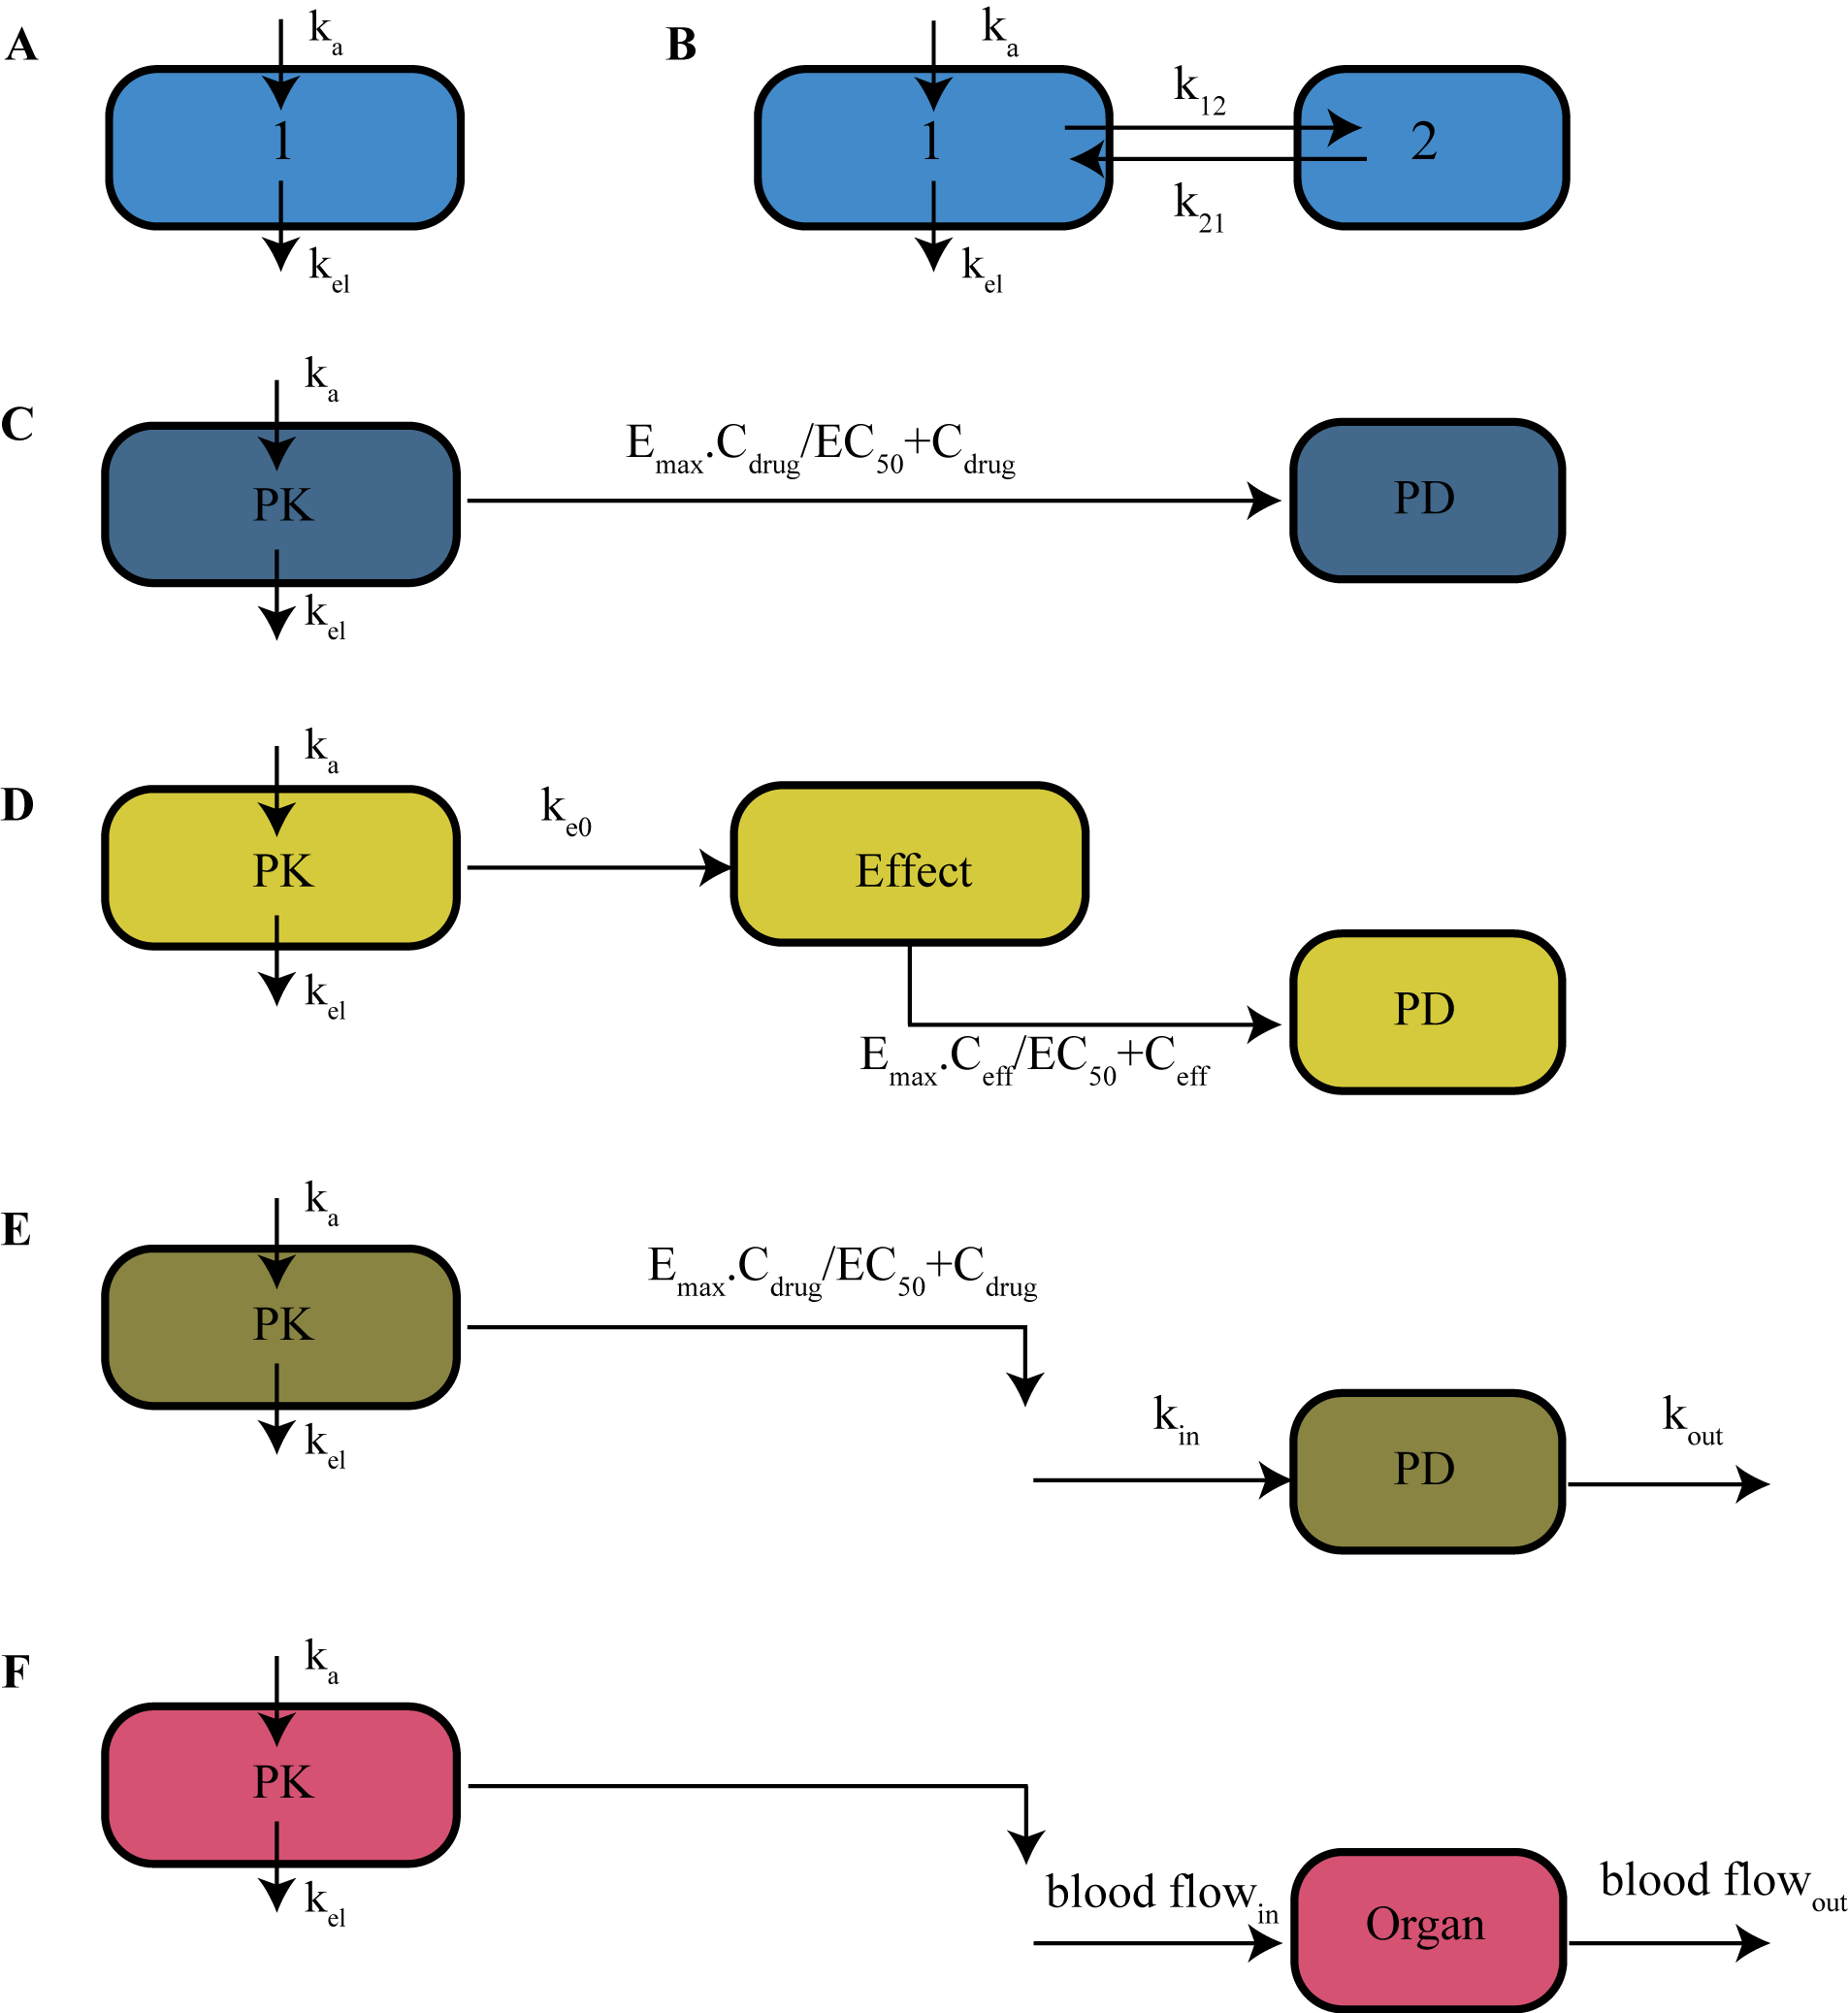
\includegraphics[width=\textwidth,height=\textheight,keepaspectratio]{PKPD/pkpd.png}%Figure from images\Figure1.png
	\caption[Different types of PKPD models.]{Different types of PKPD models. A- Monocompartmental PK model, B- Bicompartmental PK model, C- Direct effect PD model, D- PD model with effect compartment, E- Indirect effect model, F- Physiologically based PD model.}
	\label{fig:pkpd}
\end{figure}
Before the first-in-human trials, the parameters of the equations are often unknown, or at best roughly estimated through NCA. Therefore, after fitting the PK model on drug time-course concentrations in healthy volunteers, the compound parameters are estimated through non-linear regression, providing thereby a better understanding of the properties of the compounds. Oftentimes, several models are fit on the data and consequently compared on how well they explain the data through statistical metrics such as the Akaike Information Criterion (AIC) and the Bayesian Information Criterion (BIC). Model selection compares not only models of a different set of ODEs i.e., structural models, but also models with sensibly the same ODEs with slight variations. For example, in population pharmacokinetics (POP-PK), the parameters of the classical PK models can have two components, the mean population part and the individual part. Using Non-linear mixed effect (NLME) modelling, POP-PK then allows to explain between and within-individual variability to drug response. Model selection is mainly about selecting the minimal models that explain the data best. In that sense, model reduction has to be performed through eliminating correlated parameters and the inclusion of covariates such as age, sex, and weight in drug parameters. For example, the volume of distribution increases with weight, thus it can be written as following:
\begin{equation}
V= \theta + \eta*w
\end{equation}
,where $\theta$ the population mean, $\eta$ is the individual part and $w$ is the weight.  
The solution of the ODEs with the estimated parameters allows to extrapolate the PK profiles in a larger set of volunteers or patients, in order to guide later phases of clinical trials thereby enabling optimal design of experiments.
Beyond the description of pharamcokinetics, modelling provides a support to include pharmacodynamics or in other terms: what the drug does to the body. PKPD models link pharamcokinetic models to surrogate end-points e.g., the decrease of Hb1ac with anti-diabetic drugs. The pharmacodynamic effect can be modelled in various ways, depending on the delay between the administration and effect and known biology in the site of action. In cases of fast absorption and rapid distribution, the effect is observed immediately after the administration. The pharmacodynamics (PD) can be described through a direct compartment, where the drug concentrations  are directly linked to the observed phenotype \cite{upton2014basic} (Figure \ref{fig:pkpd}-C). The direct compartment is described as follows:
\begin{equation}
\begin{gathered}
E_{drug}=\frac{C_{1}}{EC_{50}+C_{1}} \\
E = E_{base}*(1-E_{drug})
\end{gathered}
\end{equation}
,where $E$ is the measured biomarker or the surrogate end point, $E_{base}$ corresponds to the basal effect prior to the administration of the compound, $E_{drug}$ is the effect induced by the drug, $EC_{50}$ is the concentration of the drug that induces half of the maximal effect and $C_{1}$ is the plasma concentration of the drug, often represented by the central pharmacokinetic compartment. In real world cases, the drug concentrations are measured as well in target organs in animal models which enables the modelling of the site of action. In many cases, the drug reaches the site of action after a certain delay as a result of slow perfusion, a signalling transduction cascade or the metabolism of prodrugs. The effect compartment has been suggested \cite{sheiner1979simultaneous} as an intermediate step between the pharmacokinetic compartment and the direct compartment. The drug concentrations from the central compartment would be subjected to a delay in the effect compartment before transducing to the direct compartment (Figure \ref{fig:pkpd}-D). If the hysteresis between the administration and the effect can be observed in the raw data, then the following effect compartment can be proposed to model the phenomenon:
\begin{equation} 
\begin{gathered}
\frac{dC_{eff}}{dt}=k_{e0}*(C_{1}-C_{eff}) \\
E_{drug}=\frac{C_{1}}{EC_{50}+C_{1}} \\
E = E_{base}*(1-E_{drug})
\end{gathered}
\end{equation}
,where the $C_{eff}$ is the concentration of the drug in the effect compartment and $k_{e0}$ is the delay parameter usually estimated from the curve fitting process as it represents the intermediary absorption and metabolism steps before reaching the site of action. The effect compartment addresses the delays caused by pharmacokinetic constraints. Likewise, in cases of delay in the pharmacodynamic processes, the indirect effect was suggested \cite{sharma1998characteristics} to model the hysteresis where the effect is neither directly linked to the central compartment nor the effect compartment (Figure \ref{fig:pkpd}-E). The indirect effect compartment is modelled as follows:
\begin{equation}
\begin{gathered}
\frac{dE}{dt}=k_{in}-k_{out}E
\end{gathered}
\end{equation}
As an example, a target protein synthesized by a zero-order rate $k_{in}$ and degraded by a first-order rate $k_{out}$ whose synthesis is stimulated by a drug, can be modelled as following:
\begin{equation} 
\begin{gathered}
\frac{dE}{dt}=k_{in}(1+E_{max}\frac{C_{eff}}{C_{eff}+EC50})-k_{out}E
\end{gathered}
\end{equation}
Symmetrically, different versions of the indirect compartment can model the inhibition and stimulation of the synthesis and degradation of the target. Generally, pharmacodynamic models exist in a wide variety of instances to describe various drug mechanisms. The pharamcokinetics of biologics for instance directly depend on their binding to the target. In this case, the pharamcodynamics drive the pharamcokinetics through target-mediated drug disposition (TMDD) models \cite{dua2015tutorial}.\\
Finally, PKPD models allow to give insights into drug effects in relation to their pharmaokinetic properties. Coupled models of pharamcokientics and pharamcodynamics allow to fit simultaneously the collected data of drug concentrations and their effect such as the target and biomarker concentration or a given clinical or physiological end point. The parameters of PKPD models are often a statistical representation that best reflect the goodness-of-fit of the model on the data. When the physiology of the system is better characterized, physiologically-based models replace the statistical parameters with mechanistic ones, thereby representing in greater detail the actual biology of the target system.
\subsection{Physiologically-based pharmacokinetic modelling (PBPK)}
PKPD models are statistical depictions of the pharmacological processes that are employed to predict drug disposition beyond the trial individuals and to guide future experiments. As such, PKPD models are rather phenomenological and lack appropriate representation of the biological system and the mechanism of drug action. In contrast, PBPK models were developed in order to go beyond the statistical representation as they integrate the known physiology of the studied system \cite{jones2013basic}. The physiological models are based on the description of human organs as compartments modelled by their weights, volume, and blood perfusion rate. Mainly used in toxicology in the beginning \cite{andersen2005introduction}, PBPK models were able to address the distribution of compounds in the different organs and assess the extent of the exposure to a given molecule \cite{peters2012physiologically}. In modelling of pharmacological agents, the PD compartments of classical PKPD model can be modified to account for known perfusion parameters in the tissue of interest giving rise to semi-physiological models \cite{wang2008preclinical} (Figure \ref{fig:pkpd}-F). The full integration of PBPK model in drug disposition uses detailed compartments of organs, where the drug absorption is modelled as following:
\begin{equation} \label{eq:PKPD}
\begin{gathered}
\frac{dC_{T}}{dt}=\frac{rate_{in}-rate_{out}}{V_{T}}\\
rate_{in}=Q_{T}C_{A}\\
rate_{out}=Q_{T} \frac{C_{T}}{K_{p}/B:P}
\end{gathered}
\end{equation}
,where $C_{T}$ is the drug concentration in the tissue, $Q_{T}$ is the blood perfusion of the tissue, $V_{T}$ is the volume of the tissue, $C_{A}$ is the arterial concentration of the drug, $K_{p}$ is the tissue to plasma partition coefficient, and $B:P$ is the blood to plasma ratio that indicates the free fraction of the drug in the plasma. The human body with its different organs modelled as compartments is represented through a generic whole-body (WB) model  \cite{peters2008evaluation} (Figure \ref{fig:s1levo}-C), that can be further expanded for the requirements of distribution of a specific drug. The basic description of each organ is based on the modelling of the in-flow of the compound through the blood perfusion, its metabolism in the organ, and the out-flow through the circulation (Equation \ref{eq:PKPD}). Additionally, several organ models \cite{poulin2002prediction,poulin2000priori,poulin2001prediction} were suggested to predict the organ-specific distribution and the concentrations of drugs in the tissue, taking into account the composition in phospholipids, neutral lipids, water, and the interstitial fraction combined with compound-specific parameters such as molecular weight, pKa, and permeability. The inclusion of these models in WB-PBPK allowed to accurately estimate the tissue to blood partition coefficient and the kinetics of the free fraction of drugs in the plasma using solely \textit{in vitro} data \cite{rodgers2006physiologically,rodgers2005physiologically,poulin2015paradigm}.
Furthermore, detailed description of the physiology of a particular system can be embedded in the WB-PBPK model such as the gastrointestinal tract that can be further compartmentalized into lumen and epithelieum as well as the different anatomical parts of the organ \cite{ando2015new,cong2000new}.\\
PBPK-PD models \cite{kuepfer2016applied} additionally include in the organ compartments the pharmacodynamics of the drug, where the drug interacts with organ specific pathways and processes. The power of PBPK models resides in the estimation of the human pharmacokinetics based mainly on \textit{in vitro} data. The \textit{in vitro}-\textit{in vivo} extrapolation (IVIVE) \cite{yeo2013application} is of paramount importance in the translation process from preclinical to clinical phases to ensure the safety of human trials \cite{lippert2012mechanistic,thiel2017comparative} and the dosing scheme for optimal efficacy. The emergence of PBPK modeling in pharmacology has been leveraged by the integration of PBPK models and simulation algorithms in software such as Simcyp (Simcyp, Sheffield, UK) , GastroPlus \cite{agoram2001predicting}, MATLAB Simbiology toolbox (The MathWorks, Natick, MA, USA), and PKSIM-MOBI \cite{eissing2011computational}. The latter is an open-source platform that enables modelling of pharmacological processes from the molecular level up to the population level.\\
Yet, in order to model organ-specific biology using ODEs, the lack of human parameters and unknown kinetics of the biological processes hinders the development of fully dynamic models. Constraint-based modelling of organ physiology using transcriptomic, proteomic, and metabolic data, can be coupled to PBPK models using dFBA frameworks to either serve as a pharmacodynamic endpoint, or to model the pharmacokinetics.
\section{Combining COBRA and PBPK}
Because of the challenges pertaining to the development of dynamic genome-scale models \cite{gilbert2017towards}, hybrid models of biological systems that encompass continuous (ODE) and discrete (FBA) behaviour, have been described in bacteria \cite{covert2008integrating,karr2012whole}, and paved the way towards kinetic genome-scale models. Combining two formalisms has the advantage of increasing the coverage of reactions, metabolites and phenotypic prediction, in addition to the temporal dimension (Table\ref{tbl:pbpkvscobra}). Moreover, additional constraints can arise from the combined model, thereby reducing the space of possible phenotypes to biologically relevant ones. Recently, the approach have been applied to human physiology through the integration of human hepatocyte metabolic model with an ODE-based PBPK model of allopurinol \cite{krauss2012integrating} to investigate the effect of enzymopathies on ammonia detoxification in the liver and the reduction of uric acid production following allopurinol treatment. Hybrid PBPK-COBRA models \cite{conde2016constraint,maldonado2017integration} were also applied in the study of phenytoin and estradiol drug-drug interaction \cite{sier2017linking}. Combined PBPK and COBRA models are anecdotic, but we expect their number and applications to extend in the community with the development of methods and tutorials.
There are two ways of constructing hybrid, bi-formalism models.

\begin{table}[h]
\caption[Comparison of PBPK models with metabolic models.]{Comparison of PBPK models with metabolic models.}
\begin{center}
	\begin{tabular*}{\textwidth}{l @{\extracolsep{\fill}} lll}
	\hline
	Model	   & PBPK                     & COBRA \\ 
	\hline
	Coverage   & a few metabolites        & genome-scale \\
	Dynamics   & dynamical                & steady state \\
	Prediction & quantitative             & semi-quantitative \\
	Parameters & many                     & few \\
	Concept    & Top-down (curve-fitting) & Bottom-up (network reconstruction) \\
	\hline
	\end{tabular*}
\end{center}
\label{tbl:pbpkvscobra}%descriptive label to refer to figure in text
\end{table}

\subsection{COBRA as pharmacodynamics - horizontal coupling}
The foundations of systems pharmacology were built on the promise of integration of systems biology models as pharamcodynamic endpoints in PKPD models \cite{iyengar2012merging,danhof2016systems}. Pharamcodynamics defined as `what the drug does to the body` would link drug concentrations to the surrogate end point and would be represented in PKPD models through phenomenological equations. Coupling COBRA models as pharmacodynamics in PBPK-PD models implies that the PK of the drug is deterministic for the entire simulation time. The coupling is considered hierarchical as concentrations from the PK compartment will shift the states of the COBRA model through time e.g., the detoxification of ammonia using a genome-scale network of the hepatocyte \cite{krauss2012integrating}. Also referred to as indirect coupling \cite{krauss2012integrating}, the method requires the identification of contact points between the PBPK-PD model and the COBRA model. Assuming that reaction $R1$ is modeled in both the PBPK and COBRA model, the method consists of solving the ODEs for each time step and subjecting the derivative terms as constraints in the metabolic model. In the PBPK model, the concentrations of metabolite $M$ are determined by a production term $v_{d,R1}$ and consumption terms $v_{d,R2}$ and $v_{d,R3}$ such as the following:
\begin{equation} \label{intro:eq1}
\frac{dM}{dt}=Mv_{d,R1}-Mv_{d,R2}-Mv_{d,R3}
\end{equation}
,where $d$ stands for dynamic.
The COBRA model is dynamically constrained for each time step and $Mv_{d,R1}$ is set as a bound in the counterpart of $v_{d,R1}$ which is $v_{m,R1}$, where $m$ stands for metabolic.
\begin{alignat*}{2}
  & \text{max or min: } &  & c^{T}v_m\\
  & \text{subject to: } &  &  
                \begin{aligned}[t] \\
                & Sv_{m}=b \\
                & v_{m,R1} \leq,=,\geq Mv_{d,R1}\\
                & v_{m,min} \leq v_{m}  \leq  v_{m,max}
                \end{aligned}
\end{alignat*} 
In most cases, the rates of absorption of the drug and its metabolites would be the most straightforward flux to couple. The PBPK-PD endpoint could be a signalling cascade involving metabolic enzymes, whose concentrations could set the upper bounds in COBRA models. While the coupling will preserve the pharmacokinetic profile of the drug, the COBRA model would have several states induced by dynamically changing the bounds of reactions in FBA programs, thereby tracking the activation of metabolic pathways over time, as an effect of the drug (Figure \ref{fig:couplings}-A). 
\subsection{COBRA as pharmacokinetics - vertical coupling}
\begin{figure}[!htp]
\centering
	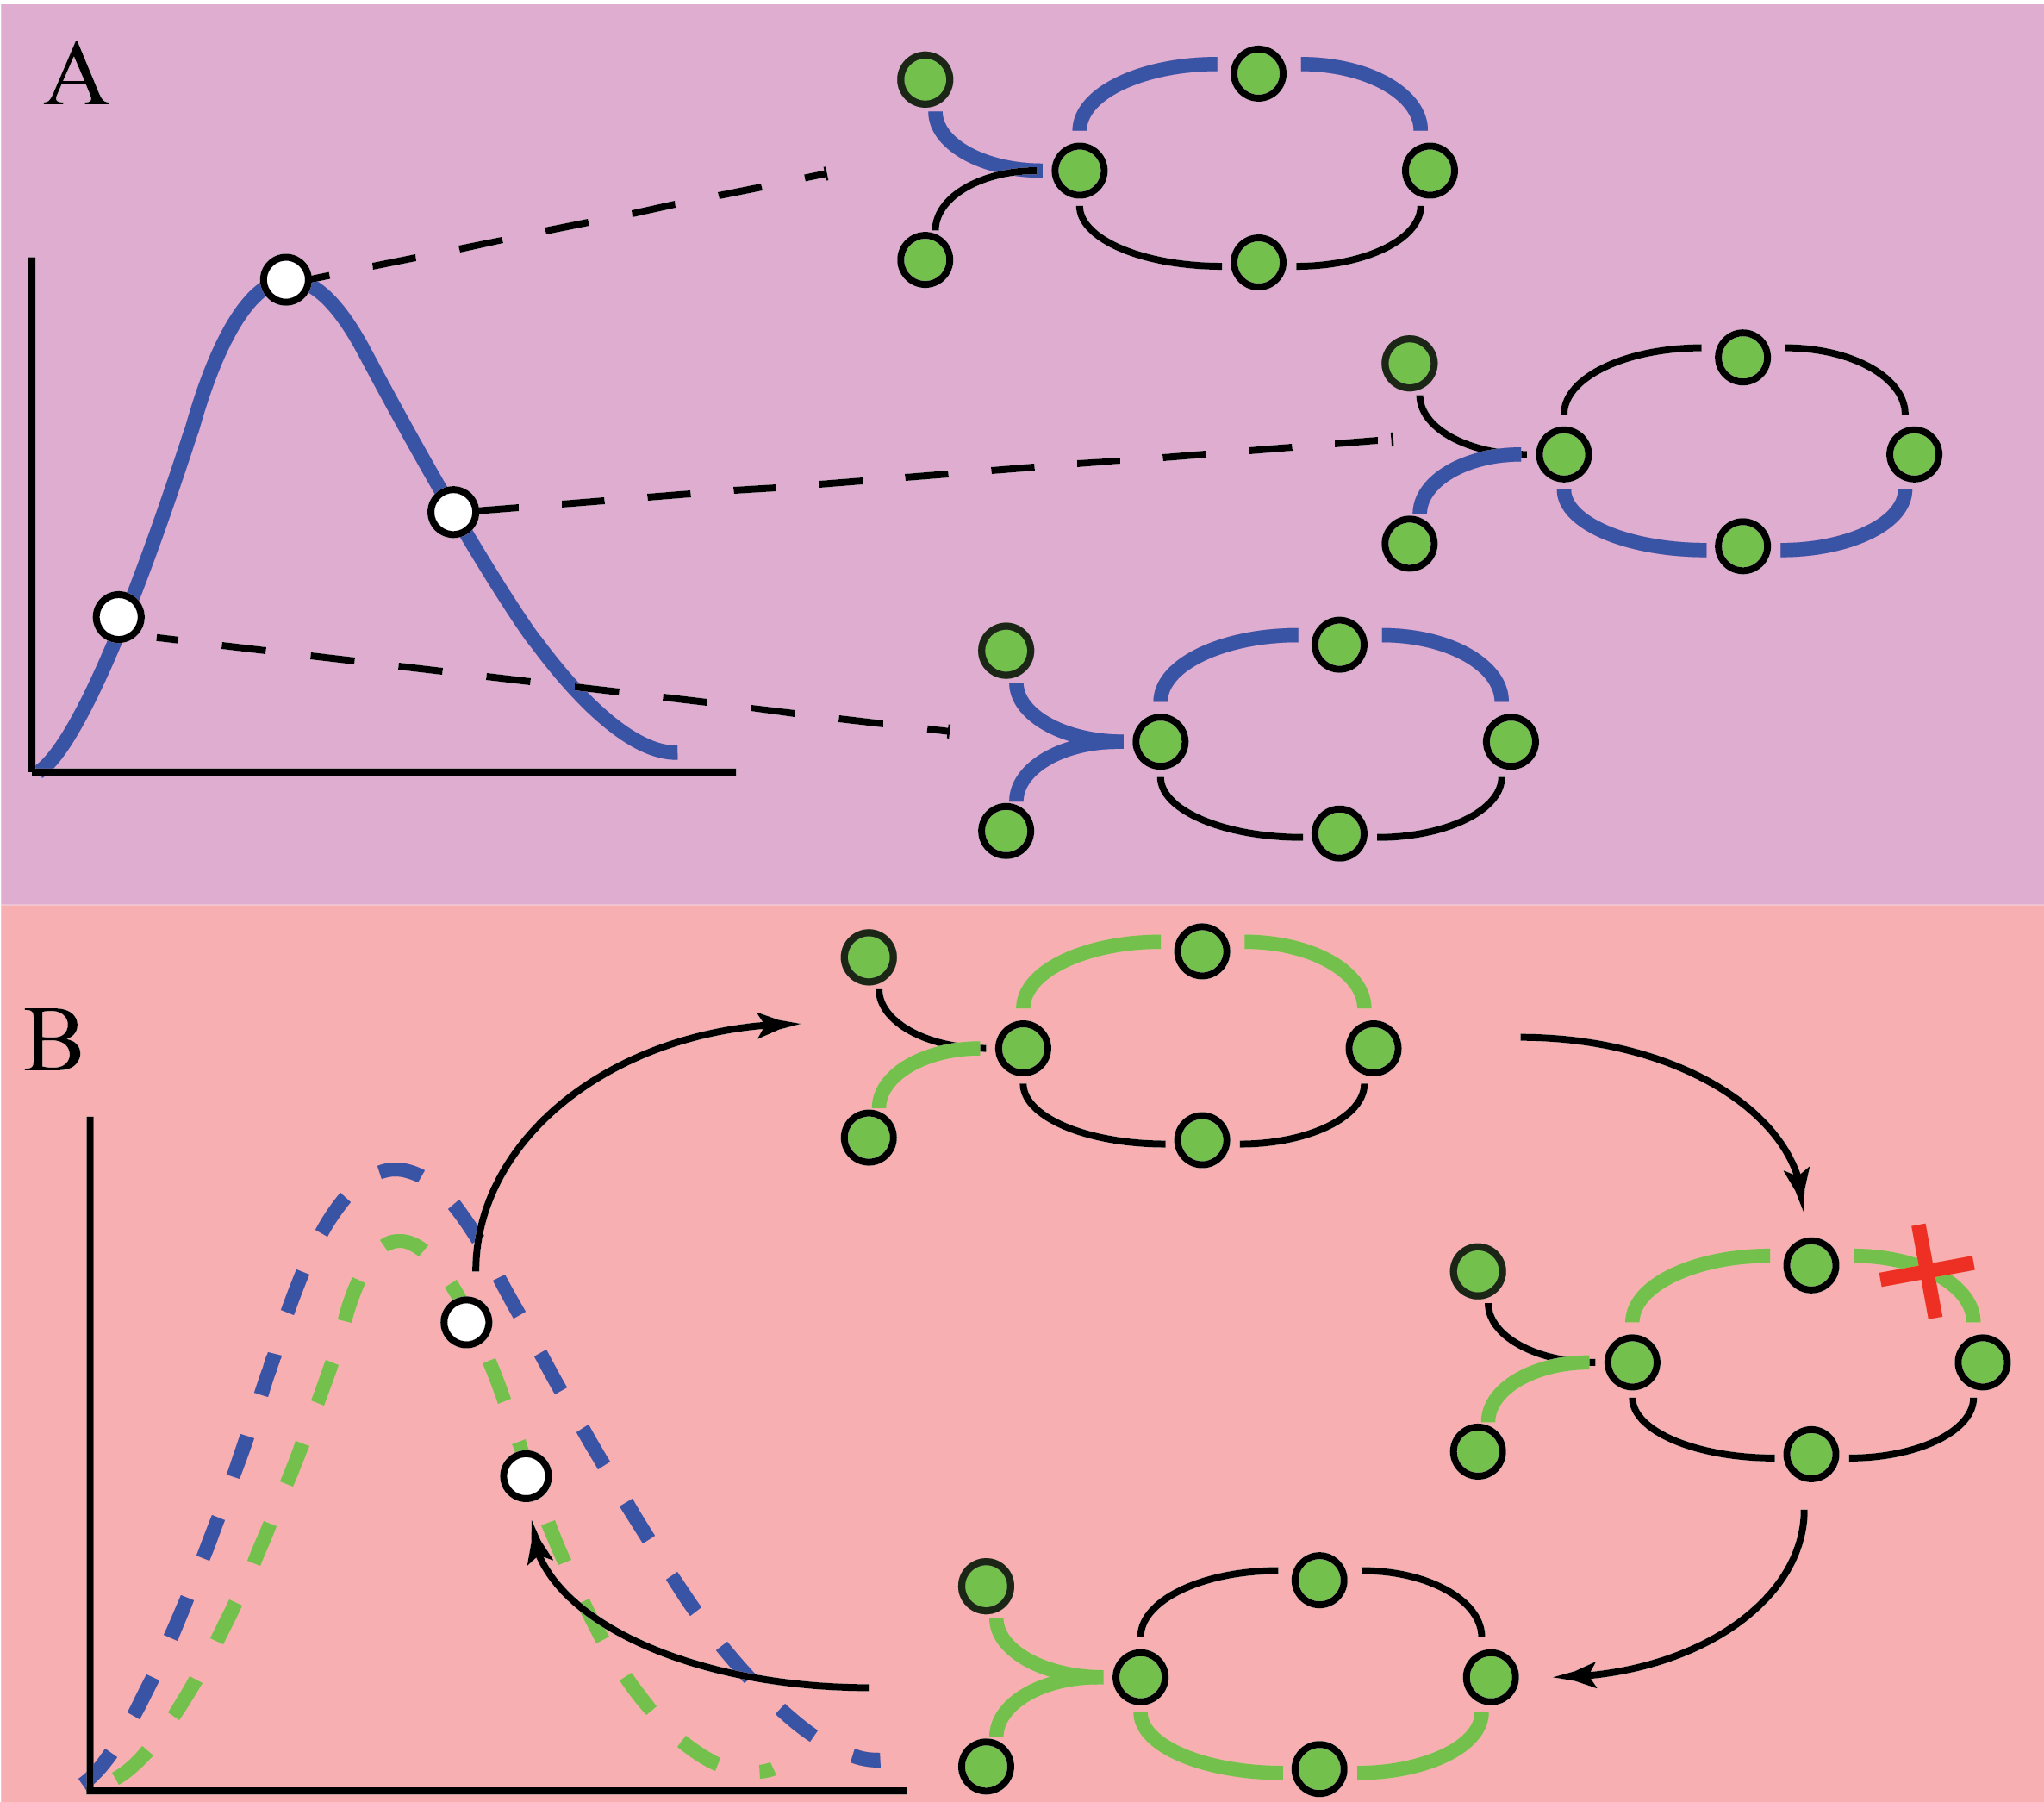
\includegraphics[width=\textwidth,height=\textheight,keepaspectratio]{Intro/couplings.png}%Figure from images\Figure1.png
	\caption[Coupling PBPK and COBRA models.]{Coupling PBPK and COBRA models. A– Horizontal hierarchical coupling consists of solving the PBPK model first in discrete time steps and subjecting reaction rates as constraints in the COBRA model to track the metabolic shift in the network as an effect of drug constraints. Depending on the research question, reaction constraints can be set as lower or upper bounds. B- Vertical coupling assumes a cross-talk between both models. As such the PK profile of the drug is not determined by the ODEs alone. In the first step, after solving the PBPK model, the derivatives are applied as constraints in the COBRA model. Additional constraints are set to represent a specific condition that is not captured by the ODE, such as enzymatic deficiency. The COBRA model is solved to obtain a solution satisfying the constraints. Finally, derivative terms in PBPK corresponding to reactions in the COBRA model solution are set accordingly and the PBPK model is integrated for the next time step. The PK of the drug obtained from the PBPK model is drawn in blue and its new PK constrained by the PBPK-COBRA model is represented in green.}
	\label{fig:couplings}
\end{figure}
Practically, hierarchical coupling would require more than one constraint to induce a shift in the steady state of the COBRA model. Since PBPK models describe usually the drug and its metabolites, additional constraints arising from gene expression experiments or metabolomics could be added to further inform the model \cite{willemsen2015metdfba}.\\
When drug pharmacokinetics are modulated by the COBRA model, as in the case of a decrease in the drug metabolising enzyme (DME) activity in the liver, enzymopathies, or in cases where the interaction with the target influences the PK as in TMDD, the coupling would be direct.
To illustrate the method, let us consider the previous PBPK model and a COBRA model sharing reaction $R1$. Solving the ODEs in the first time step allows to compute the term $Mv_{d,R1}$ corresponding to the flux of $R1$. In the COBRA model, $Mv_{d,R1}$ is set as an upper bound in the counterpart of $v_{d,R1}$ which is $v_{m,R1}$. Additional constraints could be added, such as blocking $v_{m,R6}$ to model an enzymopathy.
\begin{alignat}{2}
  & \text{max or min: } &  & c^{T}v_{m}  \label{intro:eq2}\\
  & \text{subject to: } &  & \nonumber
                \begin{aligned}[t] \\
                & Sv_{m}=0 \\
                & v_{m,R1} \leq Mv_{d,R1} \\
                & v_{m,R6} = b \\
                & v_{m,min} \leq v_m \leq  v_{m,max}
                \end{aligned}
                \nonumber
\end{alignat} 
Solving problem \ref{intro:eq2} allows to obtain $v_{m,R1}$ which sets a new value for $v_{d,R1}$ under the specified enzymopathy constraints and the ODEs \ref{intro:eq1} are integrated for the next time step.\\
The concentration time-course of the drug in the hybrid model is different from the PK profile predicted by the set of ODEs alone (Figure \ref{fig:couplings}-B). The method was described in the prediction of ammonia detoxification in patients presenting urea cycle disorder \cite{krauss2012integrating}, where the PBPK model described the PK processes of ammonia combined with a COBRA model of the hepatocyte whose ornithine carbmylase flux was gradually decreased to describe the progression of the disorder, allowing the prediction of  the PK of ammonia in patients. Another coupled model predicted alcohol concentration in volunteers who presented different alcohol dehydrogenase enzyme activity \cite{toroghi2016multiscale}. In type 1 diabetes (T1D), a PBPK model of glucose-insulin-glucagon interplay was coupled to a multi-cellular model of a myocyte, hepatocyte and adipocyte, where the impairment of T1D-related genes influenced the time-course of glucose \cite{wadehn2016multiscale}.   
We applied this approach to predict the gastrointestinal absorption of levodopa under dietary constraints wherein the presence of amino acids would induce either luminal competition or basolateral trans-stimulation, which gave rise to complex PK profiles depending on the diet composition and the time of intake \cite{guebila2016model}.
As the models include several organs and describe several metabolic processes, the issue of the non-uniqueness of solution and the non-smoothness of PK profile have been addresses through reducing the AOS space with a secondary objective (pFBA) \cite{toroghi2016multi}.\\
Taken together, COBRA models can extend the pharmacodynamics of PBPK models through a genome-scale coverage of metabolites and reactions. They alternatively can be used to predict the kinetics of the drug under new constraints arising from cellular processes such as enzymopathies. 
The inclusion of PKPD modelling, constraint-based modelling, and hybrid models under the umbrella of systems pharmacology \cite{van2011systems} has the potential to leverage the drug development process through increasing our understanding of disease pathophysiology and drug mechanism.
\section{A new drug development paradigm}
The target discovery and drug development process has been through several paradigm shifts. In the second half of the twentieth century, target discovery in the preclinical stage was driven by empirical observation on animal models, where a set of compounds were screened on disease animal models such as cancer. Rodents carrying patient-derived tumour xenograft were tested for a number of compounds and the dose was selected through titration methods. If the xenograft shrinks in size, then the compound had higher chances of translation into the clinical phases with little known about its mechanism and the reasons of success or failure. Later, the advent of crystallography and the availability of cytoplasmic and transmembrane protein structures that formed the majority of drug targets, allowed the development of the key-lock paradigm \cite{medina2013shifting}. Small molecules that fit in specific binding pockets of target proteins to induce a stimulatory or inhibitory effect, were designed through docking experiments. Computer-aided drug design and molecular dynamics are a powerful tool towards rational and optimal drug design. Nonetheless, this target-centric approach failed in considering the biological system as a whole and the selective inhibition of important signalling hubs induced long lasting side effects. Notably, Cyclooxygenase 2 (COX-2) inhibitor Rofecoxib indicated as an-inflammatory agent induced high risk of heart failure and provoked up to 30,000 deaths post-marketing between 1999 and 2004 \cite{juni2004risk}. At the same time, biology and pharmacology became data-intensive disciplines following the development of sequencing techniques \cite{lander2001initial} and the availability of data in public databases. The post-genomic drug discovery and development process has to build on known biology and fundamental science through integrating the different layers of information into convergent, hypothesis-free models of the target system \cite{van2016taking}. In line with recent calls to build model-based drug-development process by regulators \cite{us2004innovation} and by academics \cite{oberhardt2013metabolically,van2011systems}, we propose a novel drug discovery and development paradigm that builds context-specific dynamical metabolic models of human disease through transforming publicly available data into queriable knowledgebases. In the following, I will detail the vision entailed by a novel, data-intensive, model-based drug development process (Figure\ref{fig:newparadigm}) and provide examples applicable in preclinical and clinical phases using the work I carried during the course of my PhD.
\subsection{Preclinical phase}
\subsubsection{Disease signatures as targets}
The main outcome of sequencing technologies in human disease was the discovery of single nucleotide polymorphisms (SNPs) related to disease using thousands of genome wide sequences of healthy individuals and patients. Yet, GWAS studies showed that i) most of these SNPs were in non-coding regions of the genome wherein a small number of diseases could be linked to the change of sequence or structure of an enzyme, and ii) they were able to provide disease signatures. Specifically, disease signatures correspond to the gene expression profile in a given condition. Similarly, drug-induced gene expression experiments provided the gene expression related to a perturbation induced by a small molecule. Notably, the connectivity map \cite{lamb2006connectivity,subramanian2017next} has over 1.7 million \textit{in vitro} drug and drug-like induced gene expression profiles in different cell types, at different doses and different time points. Conceptually, if the drug-induced gene expression profile reverses the gene expression induced by a disease, then it can be a potential candidate for further development. For example, the reverse transcription concept has been used to treat dyslipedimia in mouse models \cite{wagner2015drugs} and repurpose drugs in nephropathy \cite{zhong2013renoprotective} and in small cell lung cancer \cite{jahchan2013drug}. Particularly, it presents a potential avenue for repurposing the existing drugs on the market for new indications \cite{dudley2011exploiting}. The clinical phase would then start directly in phase two, accelerating considerably the process and reducing the costs. Using molecules existing in the market allows to use the post-marketing safety data to reduce the amount of clinical experiments performed.
Moreover, building context-specific metabolic models of drug and disease through combining gene expression with biochemical networks allows to get insight into the phenotype of interest and predict metabolic biomarker thereby providing a rationale for the optimal design of experiments. 
\subsubsection{Target-free drug repurposing and reclassification}
The current drug classification system is based on the indication and the chemical class of the compound. The indication of the drug is oftentimes suggested prior to the beginning of the drug development program. If the drug proves to be active towards the clinical indication then it will be classified in the family of compounds that have similar activities such as the antibiotics class and the antidepressants class. Although in reality, small molecules have more than one activity. The current classification is biased towards the indication tested and intended for in the preclinical phase. The repurposing of Sildenafil and Minoxidil in erectile dysfunction and hair loss respectively, showed that a given drug could be moved from one class to the other as in case of Minoxidil from a hypotensive agents to a dermatological agent. The classification of drugs has to take into account their molecular, genetic and biochemical profile. Such classification will enable to use compounds in the same class exchangeably in similar indications, thereby harnessing drug repositioning efforts. We applied this concept to reclassify drugs with respect to their gastrointestinal effects. The drug-induced gene expression profiles from the connectivity map \cite{subramanian2017next} were used to tailor generic small intestine epithelial cell models to represent the drug action on the gut wall. Then, we clustered drugs with similar metabolic profiles into sets that had a similar genome-wide fingerprint (Chapter \hyperref[ch:chapter2]{2}). Notably, the clusters did not match the usual drug classes as currently reported by medicine agencies.
\subsubsection{Prediction of gastrointestinal side effects}
Metabolic modeling combined with machine learning was applied in the prediction of drug iatrogenic effects. Using drug induced gene expression data \cite{subramanian2017next} and reported drug target \cite{knox2010drugbank}, context-specific models informed about disrupted metabolic pathways \cite{zielinski2015pharmacogenomic}, and accurately predicted the occurence of adverse reactions \cite{shaked2016metabolic}.\\
Since the oral absorption of drugs is the most common route of administration, gastrointestinal side effects are the most frequent adverse reactions. They can induce a lower compliance to the treatment and sometimes cause the treatment to stop. The accurate prediction of gastrointestinal side effects in the preclinical phase, based solely on \textit{in vitro} data can provide invaluable information about the safety of the compound and guide the decision to proceed with clinical phases. Using the connectivity map drug gene expression profiles \cite{subramanian2017next}, we built drug-constrained metabolic models of the gastrointestinal epithelium of FDA approved drugs (Chapter \hyperref[ch:chapter2]{2}). We developed a machine learning classifier that linked drug genetic and metabolic profiles to the induced side effects as reported in the SIDER database \cite{campillos2008drug} and their mechanism of action as reported by the FDA National drug code directory (NDCD). We showed that the accuracy of prediction improved in comparison to approaches that use gene expression alone. We concluded in this work, that context-specific models of metabolism, in addition to gene expression, taken as features in a machine learning classifier could accurately predict adverse reactions.\\
The integration of multi-layer biology of genetic and metabolic signatures is a powerful tool to assess the clinical symptoms induced by xenbiotics in the preclinical phase. Moving towards the clinical phases, the translation of preclinical discovery to human has been equally in addressed in the context of PBPK models \cite{thiel2017towards} and metabolic modeling \cite{blais2017reconciled}. A consensus rat and human model \cite{blais2017reconciled} allowed to highlight species metabolic differences and to predict biomarkers to 76 drugs enabling thereby the translation of preclinical findings to clinical phases. 
\begin{figure}[!ht]
\centering
	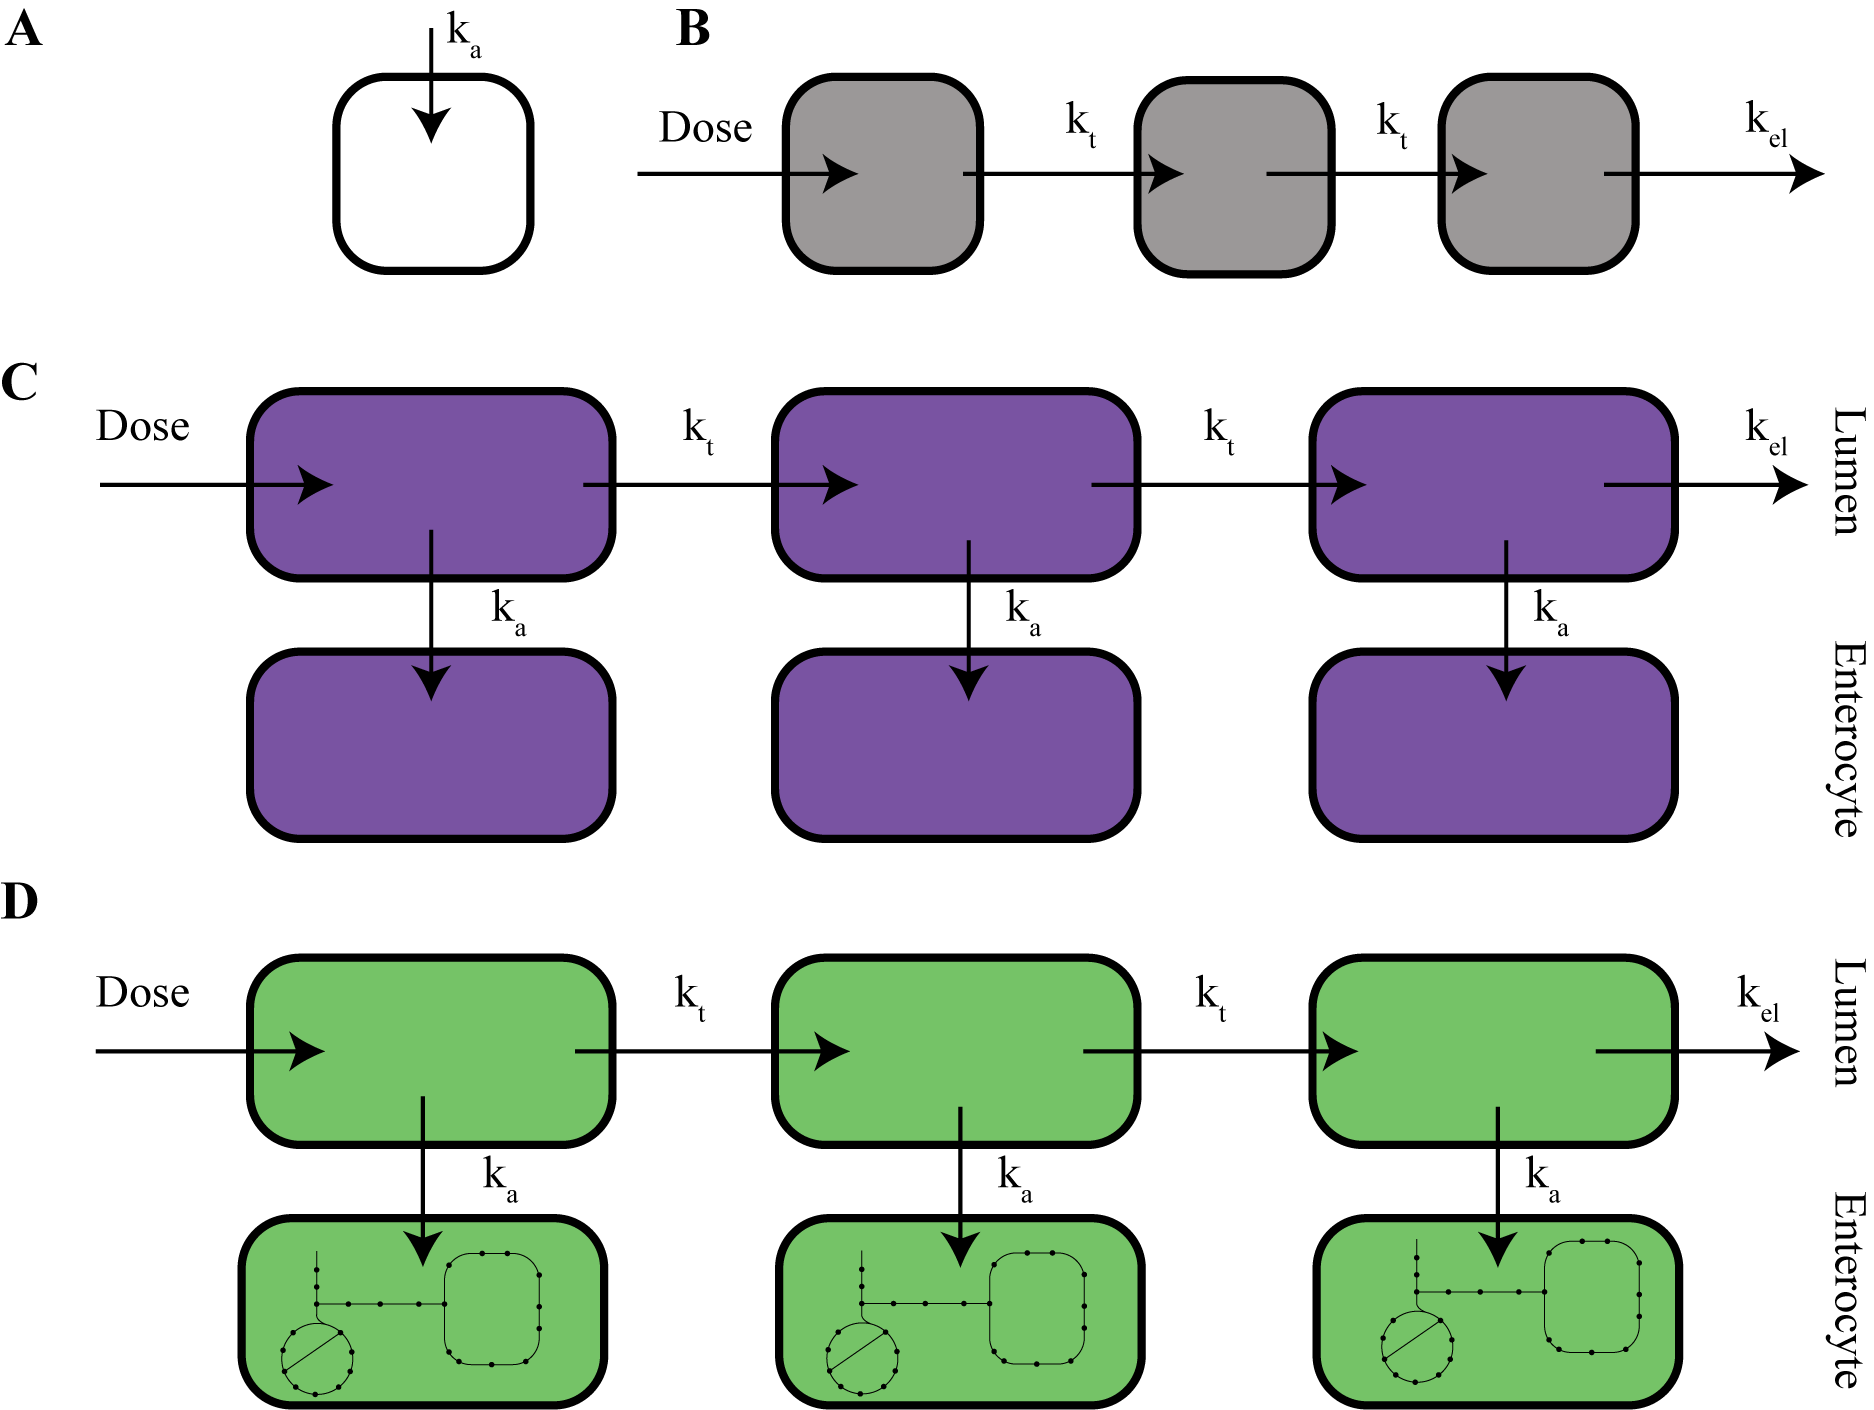
\includegraphics[width=\textwidth,height=\textheight,keepaspectratio]{ACATEVO/acatevo.png}%Figure from images\Figure1.png
	\caption[Evolution of absorption models in pharmacokinetic modeling.]{Evolution of absorption models in pharmacokinetic modeling. A- Monocompartmental PK model, B- Compartmentalized absorption and transit (CAT) model taking into account anatomical sections of the gastrointestinal tract. C- Advanced compartmentalized absorption and transit (ACAT) absorption, dissolution, and transit model. D- Small intestine epithelial cell (sIEC)-ACAT systems pharmacology model.}
	\label{fig:acatevo}
\end{figure}
\subsection{Clinical phase}
\subsubsection{Improving the bioavailability of Levodopa}
Metabolic modeling was applied in the prediction of the effects of the most commonly used marketed compounds \cite{sahoo2015modeling}. In early clinical phases, the compound is tested for potential interactions with other drugs and diet in order to optimize its efficacy and derive recommendations. As the lack of efficacy is one of the major reasons for the failure of drug development programs, we developed a gastrointestinal model to study the efficacy of a drug-diet interaction, namely levodopa and amino acids \cite{guebila2016model}. Levodopa is a supplementation therapy in Parkinson's disease, which is caused by the decrease of the amount of dopamine produced in the brain as an effect of the loss of dopaminergic neurons. The supplementation of the precursor of dopamine, levodopa, allows to restore the normal levels of dopamine in the brain. Levodopa has a similar chemical structure to amino acids, thereby it competes for absorption in the blood brain barrier and the gut wall. It is recommended for patients to avoid amino acid-rich diet to maintain the efficacy of the drug and decrease the 'on-off' phenomenon where a patient exhibits akinetic phases followed by dyskinesia. Although, the absorption of levodopa in the blood brain barrier is well documented, its transport in the gut wall was assumed to happen in a similar fashion. Recently, novel transporters of levodopa in the gut wall were identified \cite{camargo2014molecular}, which provided novel insights about the concomitant absorption of levodopa and dietary amino acids. As steady state metabolic models cannot address time-dependant phenomena, we developed a multi-scale dynamical model (Figure \ref{fig:acatevo}-D) of the absorption of levodopa along the gastrointestinal tract and we embedded a genome-scale model of the small intestine epithelial cell in the gut compartments to account for the molecular interaction between the drug and diet. We showed the mechanism beyond successful empirical dietary recommendations and provided a novel model-based diet for Parkinson's disease patients. We classified amino acids by their synergistic ability towards levodopa absorption. A recent clinical trial \cite{nagashima2016effects} showed that the absorption of levodopa was improved when soybeans were administered concomitantly, which confirmed several aspects of our hypothesis.\\
This example particularly showed the importance of the modeling-experiment loop in drug development \cite{krauss2017translational,kuepfer2012multiscale}, where the simulations integrate new findings and guide future experiments, that in return, validate the predictions and calibrate the model.
\begin{figure}[!htp]
\centering
	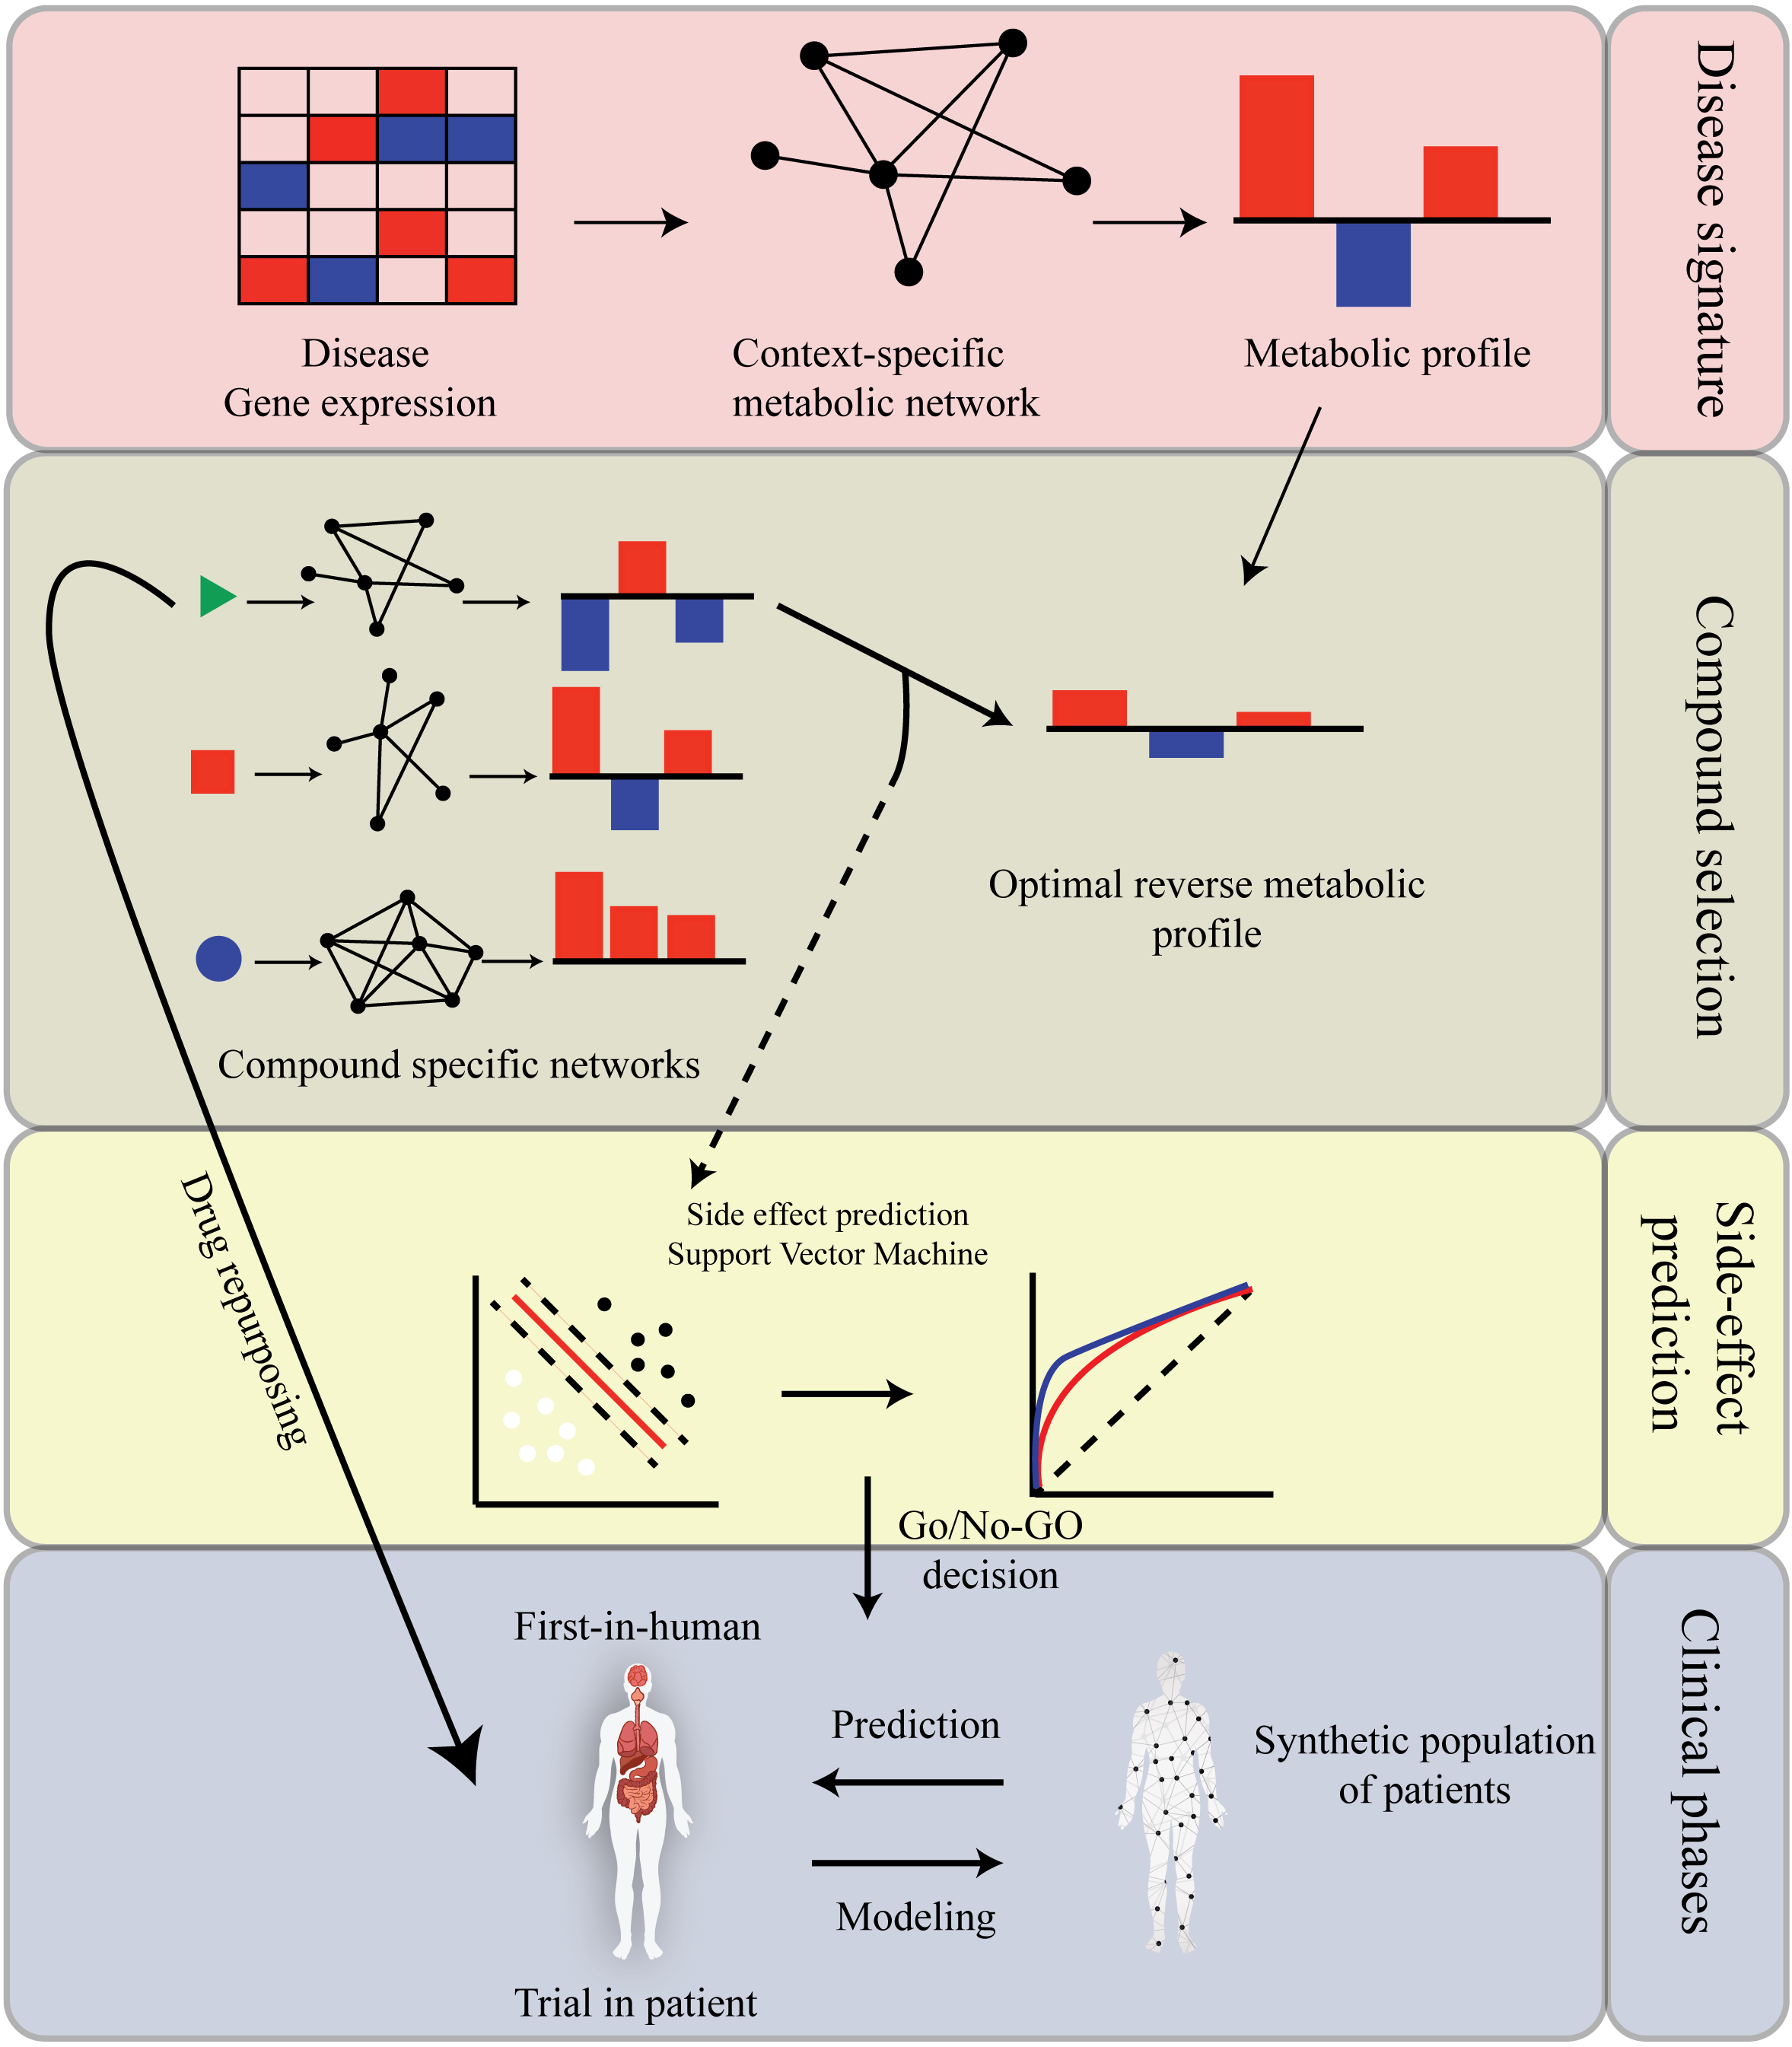
\includegraphics[width=\textwidth,height=\textheight,keepaspectratio]{NewDrugDevelopment/DrugDevPipeline.png}%Figure from images\Figure1.png
	\caption[A new drug development paradigm.]{A new drug development paradigm. Using known biology and publicly available databases, integrative disease models are built to describe the multi-layer biology of the disease. Instead of optimizing the compound for its binding affinity to a specific target, the compound is optimized for its ability to reverse the disease network state. Drug signature networks are built in a similar fashion to disease networks and compounds that reverse the systemic fingerprint of the disease are selected for further development in a target-free manner. If the small molecule exists in the market then it is moved to phase II clinical trials and repurposed for the current indication. Otherwise, the compound efficacy and safety are assessed through querying side effect databases and performing animal experiments to support the decision to move to the clinical phases. In clinical phases, an iterative approach combining empirical observation on patients and healthy individuals and the modelling of synthetic populations to guide further experiment.}
	\label{fig:newparadigm}
\end{figure}
\subsubsection{Assessing between- and within-patient response to insulin}
In later clinical phases, where the trials are expanded to a great number of participants to include several anthropomorphic groups of healthy individuals and patients, the variability of response is a major outcome of population studies which can lead to the stratification of patients through adapting the dose or deriving counter-indication for non-response groups. At this stage, clinical and molecular information about the drug is available and enables the modeling of drug pharmaockinetics in disease models \cite{danhof2015kinetics,kuepfer2010towards}. Furthermore, it can guide the large-scale experiments through modelling synthetic populations of patients. We considered type 1 diabetes as an example for this concept. Type 1 diabetes is caused by the decrease of insulin-producing cells in the pancreas, thereby causing a deregulation of the glucose-insulin-glucagon system. The onset of the disease takes place at early stages of life and requires constant supplementation of insulin to restore glucose levels. The variability of response between and within the same individual requires a constant monitoring and adaptation of the dose in addition to high socio-economical burden coming from frequent doctor visit. Type 1 diabetes being a systemic disease, we integrated a whole-body metabolic model with a dynamical model of glucose-insulin-glucagon system \cite{schaller2013generic}, gene expression data measured in T1D patients as well as the concentration time-course of key metabolites induced by insulin to build an integrated model of type 1 diabetes. We used the model to simulate a population of T1D patients and derived factors underlying inter and intra-individual variability (Chapter \hyperref[ch:chapter5]{5}). Additionally, we compared the metabolic signature of T1D to existing drug signatures and hypothesized a set of molecules as adjuvants in insulin therapy.\\
Taken together, as models of biological systems are increasing in scope and size \cite{goldberg2018emerging}, the integration of genome-scale hybrid dynamical models in all steps of the target discovery, preclinical trials, first-in-human trials to the assessment of drug-drug and drug-food interactions can leverage the drug development processes. The emergence of system-based design of therapies can optimize the outcomes and ensure higher success rates.
\section{Scope and aim of the thesis}
The project described in this thesis was built on four main objectives. First, to predict the gastrointestinal side effects of drugs based solely on \textit{in vitro} data and to classify drugs with respect to their metabolic and transcriptomic signature. Second, to predict the efficacy of levodopa under different dietary schemes using a dynamical genome-scale model of the gastrointestinal tract. Third, to design efficient computational methods in metabolic modelling to allow the simulation of large-scale metabolic models. Last, to upscale the combined models of genome-scale metabolism (COBRA) and drug disposition (PBPK) from the gastrointestinal tract to whole-body level. \\
Efficacy and safety being the two major reasons for the failure of drug development programs, I addressed the safety of compounds in the first part using drug-induced gene expression to derive context-specific models of the gut wall. I used the features of the metabolic models to predict gastrointestinal side effects and to classify drugs with respect with their metabolic and gene expression signature rather than by their indication (Chapter \hyperref[ch:chapter2]{2}). In the second part, I addressed drug efficacy with respect to a drug-food interaction specifically to optimize the gastrointestinal bioavailability of levodopa through optimizing diet using a hybrid PBPK-COBRA model (Chapter \hyperref[ch:chapter3]{3}). The third part surrounds the design of fast software for the simulation of large-scale metabolic models (Chapter \hyperref[ch:chapter4]{4}), which allows the upscaling of the combined models of metabolism and drug disposition to whole-body level. The whole-body model allowed to assess the between and within-patient variability to insulin action (Chapter \hyperref[ch:chapter5]{5}).  A brief description of the chapters and the individual contributions is provided in the following section.\\

\noindent {\large \textbf{Chapter 2: \hyperref[ch:chapter2]{Predicting gastrointestinal drug effects using contextualized metabolic models.}}}\\
\noindent Chapter \hyperref[ch:chapter2]{2} describes the prediction of gastrointestinal side effects using a statistical classifier based on \textit{in vitro} drug-induced gene expression and \textit{in silico} predicted gut wall metabolism. Then, we used genetic and metabolic features to go beyond the indication-based classification of drugs to assess compound similarities. The gut wall metabolic model was later used to assess the efficacy of the gastrointestinal absorption of levodopa (Chapter \hyperref[ch:chapter3]{3}]).
\subsubsection{Contributions}
Marouen Ben Guebila (M.B.G.) and Ines Thiele (I.T.) wrote the manuscript, M.B.G. designed the study and carried the analysis. I.T. supervised the project.\\

\noindent {\large \textbf{Chapter 3: \hyperref[ch:chapter3]{Model-based dietary optimization of late-stage, levodopa-treated, Parkinson's disease patients.}}}\\
\noindent Chapter \hyperref[ch:chapter3]{3} addresses the bioavailability of levodopa when co-administered with different types of nutritional schemes. The small intestine COBRA model was combined with a dynamical model of levodopa dynamics in the intestine (ACAT model). The combined model allowed to provide a mechanism-based diet to improve the efficacy of levodopa, which was in agreement with a recent clinical trial \cite{nagashima2016effects} . The results were published in NPJ systems biology and applications in June 2016 \cite{guebila2016model}. The chapter is a reprint of the published paper. The hybrid modeling approach was then upscaled to a whole-body level (Chapter \hyperref[ch:chapter5]{5}) through designing efficient parallel tools for metabolic modeling (Chapter \hyperref[ch:chapter4]{4}). 
\subsubsection{Contributions}
M.B.G. and I.T. wrote the manuscript and designed the study. M.B.G. carried the analysis and drew the figures. I.T. supervised the project.\\

\noindent {\large \textbf{Chapter 4: \hyperref[ch:chapter4]{Efficient parallel strategies for solving large-scale metabolic models.}}}\\
\noindent Chapter \hyperref[ch:chapter4]{4} is a description of the efficient implementation of FVA and the creation of sampling warmup points through combining message passing interface (MPI) and open multi-processing (OpenMP) parallel libraries which allowed to perform dynamical load balancing. The consequent gain in speed and memory allows to address large-scale metabolic models such as the model described in Chapter \hyperref[ch:chapter5]{5}. 
\subsubsection{Contributions}
\noindent M.B.G. wrote the manuscript. M.B.G. and I.T. designed the study. M.B.G. carried the analysis and drew the figures. I.T. supervised the project.\\

\noindent {\large \textbf{Chapter 5: \hyperref[ch:chapter5]{Pan-organ model integration of regulatory and metabolic processes in type 1 diabetes.}}}\\
\noindent The hybrid modeling approach upscaled from the gastrointestinal system to whole-body metabolism. The glucose insulin model (GIM) of glucose dynamics \cite{schaller2013generic} was coupled to Harvey, the organ-resolved human metabolic model to assess the between and within patient variability to insulin response and suggest co-drugs for diabetes control.
\subsubsection{Contributions}
M.B.G. and I.T. wrote the manuscript and designed the study. M.B.G. carried the analysis and drew the figures. I.T. supervised the project.\\

\noindent {\large \textbf{Chapter 6: \hyperref[ch:chapter6]{Concluding remarks.}}}\\
\noindent Chapter \hyperref[ch:chapter6]{6} is a reflection of my vision for the emergence of hybrid modeling in biomedical applications and the challenges that are facing the community with that respect.
\subsubsection{Contributions}
M.B.G. wrote the chapter.
\\
\\


